\documentclass[a4paper, UKenglish]{lipics-v2018}

\usepackage[dvipsnames]{xcolor}

\usepackage[utf8]{inputenc}
\usepackage{graphicx}
\usepackage{amssymb}
\usepackage{amsfonts}
\usepackage{amsthm}
\usepackage{wrapfig}
\usepackage{makecell}
\usepackage{xspace}
\usepackage{caption}
\usepackage{wrapfig}
\usepackage{float}
\usepackage{MnSymbol}
\usepackage{todonotes}
\usepackage{chngpage}
\usepackage{multirow}
\usepackage{comment}

\usepackage{array}

\newcommand{\myremark}[4]{\textcolor{blue}{\textsc{#1 #2:}} \textcolor{#4}{\textsf{#3}}}
\newcommand{\frank}[2][says]{\myremark{Frank}{#1}{#2}{SeaGreen}}
\newcommand{\patrick}[2][says]{\myremark{Patrick}{#1}{#2}{Plum}}
\newcommand{\maarten}[2][says]{\myremark{Maarten}{#1}{#2}{Red}}
\newcommand{\ivor}[2][says]{\myremark{Ivor}{#1}{#2}{Blue}}

\usepackage{longtable}
\usepackage{tabu}
\usepackage{multirow}

\newtheorem{condition}{Condition}
\newtheorem{conjecture}{Conjecture}
\newtheorem{observation}{Observation}

\newcommand{\etal}{\textit{et al.}\xspace}

% macro for making mathcal definitions
\newcommand{\mkmcal}[1]{\ensuremath{\mathcal{#1}}\xspace}

% common mathcal definitions
\newcommand{\G}{\mkmcal{G}}
\newcommand{\Lst}{\mkmcal{L}}
\newcommand{\T}{\mkmcal{T}}
\newcommand{\C}{\mkmcal{C}}
\newcommand{\X}{\mkmcal{X}}
\newcommand{\D}{\mkmcal{D}}
\newcommand{\M}{\mkmcal{M}}
\newcommand{\E}{\mkmcal{E}}
\newcommand{\BB}{\mkmcal{B}}
\renewcommand{\S}{\mkmcal{S}}
\renewcommand{\H}{\mkmcal{H}}

\newcommand{\geod}{\pi\xspace}

% macro for mathbb definitons, for definiton of the naturals N, and booleans
\newcommand{\mkmbb}[1]{\ensuremath{\mathbb{#1}}\xspace}

\newcommand{\R}{\mkmbb{R}}

\def\polylog{\operatorname{polylog}}

\title{Trajectory Visibility}
\titlerunning{Trajectory Visibility}


\author{Patrick Eades}{University of Sydney}{patrick.eades@sydney.edu.au}{}{}
\author{Ivor van der Hoog}{Utrecht University}{i.d.vanderhoog@uu.nl}{}{}
\author{Maarten Löffler}{Utrecht University}{m.loffler@uu.nl}{}{}
\author{Frank Staals}{Utrecht University}{f.staals@uu.nl}{}{}
\authorrunning{P. Eades, I. van der Hoog, M. L\"offler, and F. Staals}
\Copyright{Patrick Eades, Ivor van der Hoog, Maarten L\"offler, and Frank Staals}%mandatory, please use full first names. LIPIcs license is "CC-BY";  http://creativecommons.org/licenses/by/3.0/

\begin{document}

\maketitle

\begin{abstract}
    visible visible visible
\end{abstract}





\newpage


\section {Introduction}

\subparagraph {Trajectories.}

A \emph {trajectory} is a 
sequence of time-stamped locations 
in the plane, or more generally in $\R^d$, which
models the movement of an entity.
Trajectory data is obtained by tracking the movements of e.g. animals \cite{BovetB88,Calenge200934,gal-nmibc-09}, hurricanes \cite{Stohl1998947}, traffic \cite{lltx-dftf-10}, or other moving entities \cite{dwf-rpm-09} over time.
Large amounts of such data have recently been collected in a variety of research fields.
As a result, there is a great demand for tools and
techniques to analyze trajectory data, and many innovative algorithmic solutions have been recently developed in computational geometry~\cite{bbgll-dcpcs-11,grsc-pcecu-07,gs-tcmrm-99,lhw-tc-07,vgk-dsmt-02}.
\maarten {Cite a survey.}

\subparagraph {Visibility.}

\emph{Visibility} is one of the most studied topics in computational geometry~\cite {moet,welzl1985constructing,POCCHIOLA1996279}.
Many different terms, like art-gallery problems, guarding, or visibility itself, have been used during the last three decades to refer to problems related to the question of whether two object are \emph{visible} from each other, amidst a number of obstacles.
and even more in adjacent fields such as computer graphics~\cite {Durand00amultidisciplinary}, Geographic Information Science (GIS)~\cite{FM03}, and robotics~\cite {moet}, to name just a few.
Within computational geometry, Gosh and Giswani compiled a survey of {\em unsolved} problems in this area~\cite {Ghosh:2013:UPV:2543581.2543589}.
Buchin~\etal recently studied visibility between {\em uncertain} points~\cite {bkls-rbavil-19}, and as a subroutine solve the question of whether two points can see each other (improving an earlier result by Rote~\cite{r-dc-13} from $O(n^9)$ time to $O(n^2)$).

\subparagraph {Trajectory Visibility.}

A natural question to ask, with numerous applications, is whether two entities following different trajectories in a scene with obstacles that block visibility, can see each other.
Somewhat surprisingly, given the amount of research in both trajectories and visibility, almost no previous work in this direction exists.
Part of the reason may be that studying trajectories in {\em context} is still relatively new area, and context is essential for meaningful question.
On the other hand, the role of {\em time} is essential in this scenario: we are not interested whether there exists visibility between two geometric shapes, but rather whether there exists a {\em time} at which two point objects are visible. This makes the question fundamentally different from existing work in visibility.

\subparagraph {Variants.}

Trajectories walk through walls or not?
Include figure.



\subparagraph {Data Structures.}

In many analysis applications, trajectories live in a static environment (the obstacles), but new trajectories arise over time. This raises the natural question whether one can store the environment in a data structure that can support visibility queries between trajectories.
\maarten {In a later version, we should work out some of these applications. One of them is sampling from a distribution (our original one), but I'm sure there are many other scenarios in which the environment doesn't change, but the trajectories do. :)}

Solutions for the same question for point-to-point visibility are well-known.
Guibas and Hersberger \cite{GUIBAS1989126} present a linear-size data structure on a simple polgyon which can return, the shortest path between a pair of query points in logarithmic time. Note that the points are mutually visible if and only if their shortest path is a single line segment. \maarten {Find out about earlier solutions for this problem.}

\subparagraph {Trajectory planning.}

In contrast to {\em testing} visibility between trajectories, there is a considerable body of previous work on trajectory {\em planning} under visibility contraints (points should remain mutually visible) or with the aim to maximize visibility.
Shkurti and Dudek~\cite {6907405} consider the complementary problem: how can we plan the trajectories of two moving objects such as to maximize visibility between them.
This problem is also closely related to {\em camera planning}~\cite {christie}, where one trajectory is given as input but a second one should be chosed to maintain visibility between the two points.
\maarten {Eventually we should do a more thorough review of this area.}


\subparagraph {Formal Problem statement.}

  Given a simple polygon $P$, preprocess $P$ into a data structure that can answer queries of the following type: given two trajectories $T_1$ and $T_2$ that represent the motion of two moving entities $e_1$ and $e_2$ within $P$, is there a time $t^*$ at which $e_1$ and $e_2$ see each other?
    
\maarten {Unify notation.}

\subparagraph {Results.}

  If we denote by $n$ the complexity of $P$, and by $m$ the total complexity of the two query trajectories, we obtain the following result:
  
  We can preprocess $P$ in $O(...)$ time into a data structure using $O(...)$ space, such that a query can be answered in $O(...)$ time.



\section{Introduction}

In a geometric context, two objects are visible to each other if the line segment connecting them does not cross any obstacles. Visibility is a core subject within computational geometry; in the past 30 years there have been more than 500 publications \cite{ORourke87}. A trajectory is a sequence of time-stamped locations in the plane (or more generally, in $\mathbb{R}^d$). Trajectory data is obtained by tracking the movements of e.g. animals \cite{BovetB88,Calenge200934,gal-nmibc-09}, hurricanes \cite{Stohl1998947}, traffic \cite{lltx-dftf-10}, or other moving entities \cite{dwf-rpm-09} over time.
Large amounts of such data have recently been collected in a variety of research fields. As a result, there is a great demand for tools and
techniques to analyze trajectory data, and many innovative algorithmic solutions have been recently developed in computational geometry~\cite{bbgll-dcpcs-11,grsc-pcecu-07,gs-tcmrm-99,lhw-tc-07,vgk-dsmt-02}
We consider the fundamental problem linking visibility and trajectory analysis: given two entities $q$ and $r$ that each travel along a trajectory, is there any time where $q$ and $r$ can see one another? Surprisingly (given the considerable amount of research on both visibility and trajectories), this is the first paper where visibility between trajectories is considered. We provide a wide collection of results for various types of trajectories and obstacle domains, see Table \ref{tab:results}.

%\emph{Trajectory planning} is a fundamental issue for robotic applications and automotion in general \cite{gasparetto} and it is the core motivation for a large number of publications in computer science \cite{}. \patrick[wonders]{how important trajectory plannning is for us.}

\subparagraph{Visibility.}

Visibility is one of the most studied topics in computational geometry~\cite {moet,welzl1985constructing,POCCHIOLA1996279}. Various core problems of computational geometry consider the visibility between objects in an obstacle domain and we mention a few:
The ray shooting problem (given a polygon and a ray emanating from a given point in a given direction, find the first intersection, if any, of the ray with the polygon boundary) has been studied by Chazelle [10], Chazelle and Guibas [13], Guibas~\etal [17], and Hershberger and Suri [20]. The guarding problem (given a polygon, find a placement of guards at the vertices to cover the whole polygon) and its many variations has been studied by Chvatal \cite{Chvatal75}, Fisk \cite{Fisk78} and \patrick{survey}.

The visibility graph problem asks, given an object set $Q$ within an obstacle domain $P$, to construct a graph on $Q$ where two objects share an edge if they are mutually visible. The visibility graph is extensively used in robot motion planning \cite{de1997computational} and it has many variants (refer to \cite{Ghosh:2013:UPV:2543581.2543589} for a survey). The 3D variant was shown to be NP-hard \cite{canny1988complexity} and recently it has been shown that the recognition variant is $\exists \mathbb{R}$-complete \cite{cardinal2017recognition}. The visibility polygon problem (given a polygon P and a point q inside the polygon, determine the polygon consisting of all the points in P visible from q). Early results on this problem include the work by ElGindy and Avis \cite{el1981linear}, Lee \cite{lee1983visibility} and Joe and Simpson \cite{joe1987corrections}. Recent results focus on visibility polygon retrieval and include Aronov \etal \cite{aronov2002visibility}, Zarei \etal \cite{zarei2005efficient} and most recently Diez \etal \cite{DKRRS2017KineticAPSPEuroCG}.

For more information about visibility problems, refer to Appendix~$A$, O'Rourke's book \cite{ORourke87} chapter 28, and the surveys by Durant \cite{durand2000multidisciplinary} and Gosh  \cite{Ghosh:2013:UPV:2543581.2543589}. 

\patrick{This should go somewhere ...} Lee and Preparata \cite{LeeP84} find the shortest path between two points in a simple polygon in linear time, if linear time triangulation is used; which implicitly solves visibility between two points.

\subparagraph{Visibility and motion.}

Visibility of a moving object is an old subject within visibility that recently has gained attention within the computational geometry community. Bern \etal \cite{bern1994visibility} and  Mulmuley \cite{mulmuley1991hidden} study maintaining the visibility polygon of a point that moves over a straight path. 
Buchin~\etal studied visibility between {\em uncertain} points~\cite {bkls-rbavil-19}, and as a subroutine solve the question of whether two points can see each other (improving an earlier result by Rote~\cite{r-dc-13} from
$O(n^9)$ time to $O(n^2)$).  Karavelas and Guibas \cite{karavelas2001static} describe how to maintain a constrained Delaunay triangulation of a set of moving points, and show how this can be used to maintain nearest neighbors.
Aronov \etal \cite{aronov2002visibility} demonstrate a kinetic algorithm that tracks the visibility polygon of a moving query point $q$. The most recent result on visibility and motion is by Diez \etal \cite{DKRRS2017KineticAPSPEuroCG} who show how to maintain the shortest path between two moving entities using a kinetic data structure. The entities can see one another if and only if their shortest path is a line segment and thus this kinetic data structure can be used to compute visibility between two moving entities. For more information on visibility during motion refer to the summary of prior results in Appendix~$B$.

\subparagraph{Trajectories.}
A recent dramatic increase in the availability of low-cost, internet connected GPS tracking devices has driven considerable interest in spatio-temporal data (commonly called trajectories) across fields including GIScience, databases, and computational geometry. Problems relevant to computational geometry include detecting and describing flocks \cite{AnderssonGLW07, BenkertGHW08, LaubeKI04} and hotspots, clustering and categorising trajectories, map construction and \ldots.
\patrick{We can cite trajectory stuff infinitely, to what extent do we want to lit review?}

Data can come from animal tracking, car and ship traffic, pedestrian crowds, sportspeople, and abstract spaces such as political sentiment or stock prices.

Gudmundsson~\etal have a survey of the increasing importance of trajectory data in a wide variety of fields \cite{GudmundssonLW17}.

\subparagraph{Data Structures.}
In many analysis applications, trajectories live in a static environment (the obstacles), but new trajectories arise over time. This raises the natural question whether one can store the environment in a data structure that can support visibility queries between trajectories.
\maarten[has previously said]{In a later version, we should work out some of these applications. One of them is sampling from a distribution (our original one), but I'm sure there are many other scenarios in which the environment doesn't change, but the trajectories do.}
Solutions for the same question for point-to-point visibility are well-known.
Guibas and Hersberger \cite{guibas1989optimal} present a linear-size data structure on a simple polgyon which can return the shortest path between a pair of query points in logarithmic time. Note that the points are mutually visible if and only if their shortest path is a single line segment.

Guibas and Hershberger's work concludes a series of triangulation-based shortest path algorithms for a simple polygon including Lee and Preparata \cite{LeeP84}, Reif and Storer \cite{ReifS85} and Guibas~\etal \cite{GuibasHLST87}. \patrick{How deep into ancient history do we really want to go here}

\subparagraph{Problem statement and results.}

We are given a polygonal domain $P$ with $n$ vertices and we want to build a data structure that can answer queries of the type: given two entities $r$ and $q$ that move along trajectories $T_r$ and $T_q$ with $\tau$ vertices in the time frame $[0,1]$,  is there a time $t$ where $q$ and $r$ can see one another? We consider the situations where $T_r$ and $T_q$ are both points, $T_r$ is a line segment and $T_q$ is a point and $T_r$ and $T_q$ are both line segments. We consider the domains where $P$ is a simple polygon, $P$ is a simple polygon where the trajectories can go through edges and $P$ as a polygonal domain. In each of these scenarios, we preprocess $P$ to obtain sub-linear query time.The original problem can therefore be solved in $o(\tau n)$ time.  For each scenario we also provide a one-shot algorithm for comparison. In this paper we encounter the following sub-problem: given a convex polygon $P'$ with $m$ vertices, can you build a data structure such that for any hyperbolic segment $\gamma$, one can determine an intersection between $P'$ and $\gamma$ (if any exists)? We show how to preprocess $P'$ such that these queries can be solved in time sub-linear in $m$ and we believe that this result could be of independent interest. The main idea of this paper, is to transform the visibility (or intersection) queries into $k$-dimensional halfspace empyness queries for a constant dimension $k$. Throughout this paper we solve $k$-dimensional halfspace emptyness queries using the partition trees from Chan \cite{chan2012optimal} which preprocess a set of $n$ objects in $\mathcal{O}(n^{1+ \varepsilon}$ time, $\mathcal{O}(n)$ space and can answer halfspace range queries in $\mathcal{O}(n^{1 - \frac{1}{k} + \varepsilon})$ time where $\varepsilon$ is an arbitrarily small positive constant. $k$-dimensional halfspace emptyness queries can also be solved using cutting trees which use $\mathcal{O}(n^{k})$ storage and preprocessing time for a faster $\mathcal{O}(\log^k n)$ query time. So throughout the paper, you can insert this value for a time-space tradeoff.

\begin{table}[]
    \centering
    \begin{longtabu}{|c|c|c|c|c|c|c|c|}
    \hline
   \rowfont{\bfseries}
        \multirow{2}{*}{q} & \multirow{2}{*}{r} & \multirow{2}{*}{$P$} & algorithm & \multicolumn{3}{c|}{data structure} & source \\ 
        & & & & space & preprocessing & query & \\
        \hline\hline
        %
        \multirow{2}{*}{$\bullet$} & \multirow{2}{*}{$\bullet$} & S or I &  $\Theta(n)$ & $\Theta(n)$ & $\mathcal{O}(n \log n)$ & $\Theta(\log n)$ & \cite{guibas1989optimal} \\
        & & D & $\Theta(n)$ & $\mathcal{O}()$ & $\mathcal{O}()$ & $\mathcal{O}()$ & \cite{POCCHIOLA1996279} \\ 
        \hline
        %
        \multirow{3}{*}{$\bullet$} & \multirow{3}{*}{$\slash$} & S & $\Theta(n)$ & $\Theta(n)$ & $\mathcal{O}(n \log n)$ & $\Theta(\log n)$ & Section~\ref {} \\
        & & I & $\Theta(n)$ & $\mathcal{O}(n^{2} \log n)$ & $\mathcal{O}(n^{2 + \varepsilon})$ & $\mathcal{O}(n^{\frac{7}{8} + \varepsilon})$ & Section~\ref {} \\
        & & D & $\mathcal{O}(n \log n)$ & $\mathcal{O}(n^4 \log n)$ & $\mathcal{O}(n^{4 + \varepsilon })$ & $\mathcal{O}(n^{7/8 + \varepsilon})$ &  Section~\ref {} \\ 
        \hline
        %
        \multirow{3}{*}{$\slash$} & \multirow{3}{*}{$\slash$} & S & $\Theta(n)$ & $\mathcal{O}(n \log n)$ & $\mathcal{O}(n^{1 + \varepsilon})$ & $\mathcal{O}(n^{3/4 + \varepsilon})$ & Section~\ref {} \\
        & & I & $\Theta(n)$ & $\mathcal{O}(n^{c})$ & $\mathcal{O}(n^{c+\varepsilon})$ & $\mathcal{O}(\log^c n)$ & Section~\ref {} \\
        & & D & $\mathcal{O}(n \log n)$ & $\mathcal{O}(n^c)$ & $\mathcal{O}(n^{c + \varepsilon})$ & $\mathcal{O}(\log^c n)$ & Section~\ref {}\\ 
        \hline
    \end{longtabu}
    \caption{The table of results, assuming one uses partition trees. See the theorems for more general bounds. The constant $c$ is not determined but very high. The two left-most columns specify if the query entity is a point ($\bullet$) or line segment ($\slash$). The third column specifies if the domain $P$ is a simple polygon with $n$ vertices (S), a polygon where the query segments may intersect $P$ (I) or a polygonal domain with $n$ vertices (D).}
    \label{tab:results}
\end{table}
\maarten {I don't think the term "transparent" is the right one to use: to me something transparent is something I can see through but not walk through, not the other way around.}

\subparagraph{Discussion of our results}

\ivor{some story on the different variants and why they are all useful}

\section{Preliminaries}
\label{sec:prelims}

If we are allowed to preprocess $P$ we use multi-level data structures to answer the queries from Table~\ref{tab:results}. As the base level of these multi-level structures we either use the shortest path structure from Guibas and Hershberger \cite{guibas1989optimal} or the visibility polygon retrieval structure from Aronov \etal \cite{aronov2002visibility}. At the top level we transform the visibility query, into an intersection query between an algebraic query object and a pre-stored geometric object from the lower levels. We compute these intersections using linearization from Agarwal \etal \cite{agarwal2013range}.


\subparagraph{Shortest path queries.}
Two points $q,r \in P$ are mutually visible if and only if the shortest path between them is a line segment.  Guibas and Hershberger \cite{guibas1989optimal} create a $\Theta(n)$ size data structure, in $\mathcal{O}(n \log n)$ time, that can answer shortest-path queries in $P$ in $\Theta(\log n)$ time. Let $e$ and $e'$ be two edges in $P$, the \emph{hourglass} $H(e, e')$ is the union of all shortest paths from points on $e$ to points on $e'$. Guibas and Hershberger show that $H(e, e')$ is a polygon in $P$ which is bound by $e, e'$ and the shortest paths between the endpoints of $e$ and $e'$. Since an hourglass is bounded by four paths in $P$, the hourglass can be represented as a red-black tree where each node represents an edge on the border of $H(e, e')$, this is called the \emph{implicit representation}. 
Guibas and Hershberger build a balanced hierarchical subdivision of $P$ using its diagonals, where the leaves in the subdivision form a triangulation of $P$. Each node in the tree represents a subpolygon and stores several implicit hourglasses between diagonals. A shortest path query between two points $q,r \in P$ is answered as follows: they locate the leaf triangles $\Delta_q$ and $\Delta_r$ which contain $q$ and $r$. Next they identify  $\mathcal{O}(\log n)$ pre-stored hourglasses and concatenate them using at most $\mathcal{O}(\log n)$ \emph{outer tangents} to form the hourglass between $\Delta_q$ and $\Delta_r$. This hourglass can be used to find the shortest path between $q$ and $r$. Refer to Figure~\ref{fig:guibas} for an example. For polygonal domains we use the visibility complex from Pocchiola and Vegter \cite{pocchiola1996visibility} to obtain hourglass-like objects instead.


\begin{figure}[h]
    \centering
    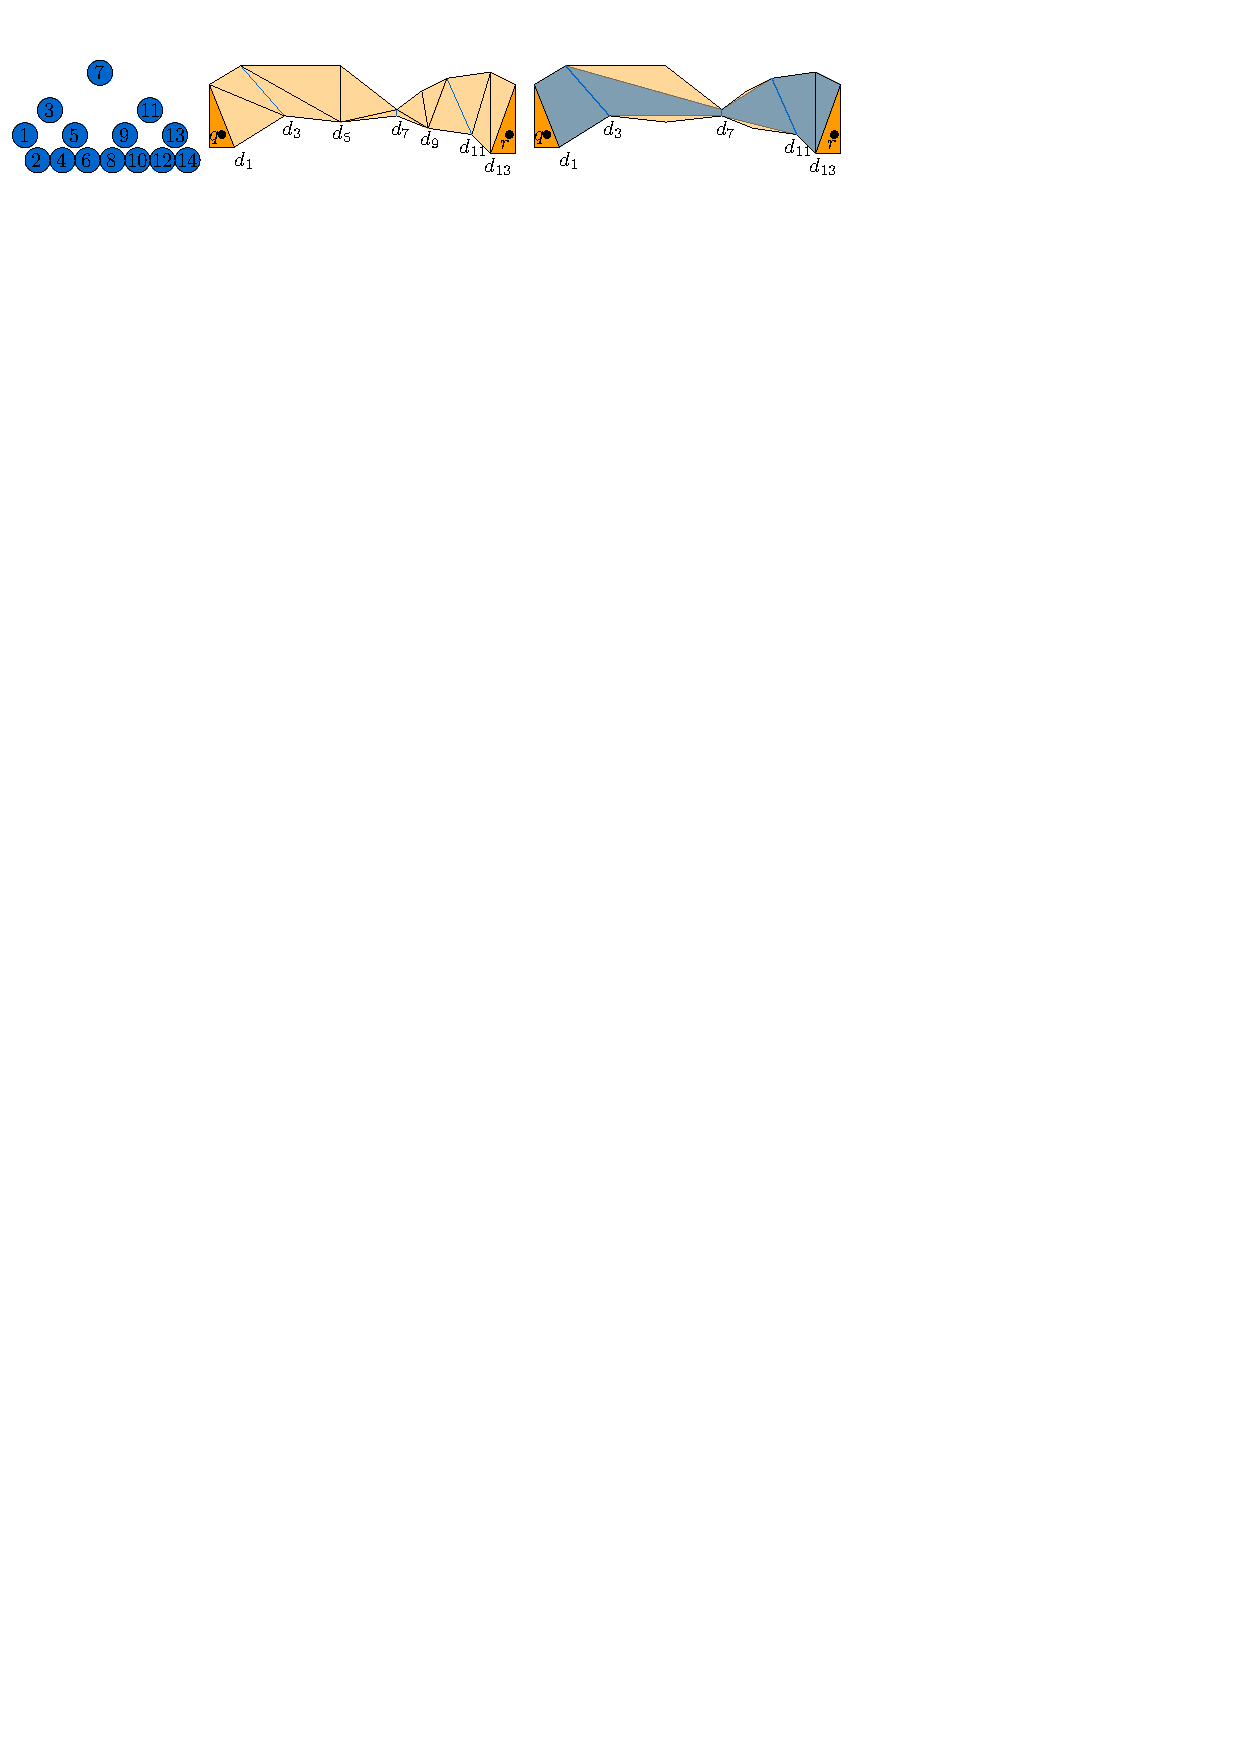
\includegraphics[]{../guibas}
    \caption{A triangulated polygon $P$ where the diagonals are labelled from $d_1$ to $d_{14}$. (left) a balanced hierarchical subdivision on the diagonals. (right) There are $13$ diagonals between $\Delta_q$ and $\Delta_r$. However, we have pre-stored hourglasses $H(d_1,d_3)$, $H(d_3, d_7)$, $H(d_7, d_{11})$ and $H(d_{11}, d_{13})$. Thus during query time, we only have to concatenate $\mathcal{O}(\log n)$ hourglasses to get $H(d_1, d_{13})$. }
    \label{fig:guibas}
\end{figure}


\subparagraph{Visibility polygon retrieval.}
For any point $q$ in a polygonal domain $P$, its \emph{visibility polygon} $V_q$ is the union of all points visible from $q$. There are two types of edges bounding $V_q$ which we call certain or uncertain. A certain edge coincides with an edge of $P$. An uncertain edge is an edge $e$ of $P$ with a corresponding reflex vertex $v_e$ of $P$. One endpoint of $e$ is the intersection between the line $qv_e$ and $e$. For all $q \in P$, the \emph{implicit} visibility polygon is a clockwise order of the certain and uncertain edges (together with their corresponding vertex) of $V_q$ , stored in a red-black tree. Aronov \etal \cite{aronov2002visibility} show how to partition a simple polygon $P$ into $\mathcal{O}(n^2)$ triangles such that for each triangle, all points in that triangle have the same implicit visibility polygon. This allows them to prepreprocess $P$ in $\mathcal{O}(n^2\log n)$ time using $\mathcal{O}(n^2)$ space, such that for any query point $q$, one can get a pointer to the implicit $V_q$ in $\mathcal{O}(\log n)$ time. We extend their approach to work for polygonal domains.





\subparagraph{Persistence.}
The aforementioned data structures create a hierarchical decomposition of $P$ and store in each node of this tree an implicit representation of a sub-polygon of $P$ (be it an hourglass or a visibility polygon) as a red-black tree. For both data structures, neighbouring nodes in the decomposition store near-identical red-black trees. A persistent data structure (introduced by Sarnak and Tarjan \cite{sarnak1986planar}) is a data structure that accepts an arbitrarily long sequence of updates, but is able to remember at any time all its earlier versions. Both data structures make use of persistence to save storage space \cite{hershberger1991new, aronov2002visibility}: instead of storing a unique tree at every node of the decomposition they store one partially persistent red-black tree  which for each adjacent node in the decomposition, remembers an update that transforms the red-black tree into the node for that tree. We make extensive use of persistence.

\subparagraph{Semi-algebraic range searching.}

Let $X$ be a set of $n$ geometric objects in $\mathbb{R}^d$, where each object is parametrized by a vector $\vec{x}$ (e.g. a point is parametrized by a vector of its coordinates). Let $\Gamma$ be a family of geometric regions (called semi-algebraic ranges) in $\mathbb{R}^d$ where each region $G \in \Gamma$ is bound by an algebraic curve $\gamma$ which is parametrized by a vector $\vec{a}$. Agarwal \etal \cite{agarwal2013range} are interested in preprocessing $X$, such that for any range $G \in \Gamma$, we can report which objects of $X$ intersect $G$. They show the following: suppose you can derive a predicate function $F(\vec{x}, \vec{a}) \le 0$ that for any object and any query (parametrized by $\vec{x}$ and $\vec{a}$ respectively) specifies if the object intersects the query.  Moreover, this function is of the form: $F(\vec{x}, \vec{a}) =  g_0(\vec{a}) + \sum_{i=1}^k g_i(\vec{a})f_i(\vec{x})$ where $f_i$ and $g_i$ are polynomials dependent only on $\vec{x}$ and $\vec{a}$ respectively. Then Agarwal \etal show how to transform this $d$-dimensional semi-algebraic range searching problem into a halfspace range searching problem into $\mathbb{R}^k$. Specifically, Agarwal \etal prove that you can map any $d$-dimensional point $\vec{x}$ to the $k$-dimensional point $f(\vec{x}) = (f_1(\vec{x}), f_2(\vec{x}), \dots f_k(\vec{x}))$, and any query range to the $k$-dimensional halfspace $G(\vec{a}) = \left\{ \vec{y} \in \mathbb{R}^k \mid g_0(\vec{a})  + \sum_i^k g_i(\vec{a})y_i  \le C \right\}$ and that $\vec{x}$ intersects $G$ if and only if $f(\vec{x})$ is contained in $G(\vec{a})$. Refer to Figure~\ref{fig:algebraic} for an example. Transforming an algebraic expression into this restricted form is called \emph{linearization} and $k$-dimensional halfspace range searching can be solved using partition trees \cite{chan2012optimal} or cutting trees \cite{chazelle1993cutting}.



\section{Intersecting a curve segment and a convex polygon}
\label{sec:intersectionsearch}

We now turn our attention to a problem which is closely related to visibility between trajectories, although the link may not be immediately obvious. The results of this section are an integral part of the data structure presented in Section~\ref{sec:lineline}. We present this problem separately for two reasons: (1) we believe the result to be of independent interest, (2) this section is a good example of the techniques that we use throughout this paper. 

Suppose we are given a set $E$ of $n$ edges which form a convex polygon $P_E$. We want to preprocess $E$, such that given any segment $\gamma$ of an arbitrary degree-2 polynomial curve in the plane, we can test whether $\gamma$ intersects $P_E$ in sub-linear time. This check can be performed easily in linear time by testing for an intersection with every edge in $E$ and checking if $\gamma$ is entirely contained within $P_E$. We assume $\gamma$ starts at the point $s$ and ends at the point $t$. Moreover we assume that the curve segment $\gamma$ coincides with a degree 2 curve $\Gamma :: a_1 x^2 + a_2 x + a_3 xy + a_4 y + a_5 y^2 + a_6 = 0$ and we denote $\vec{a} = (a_1, \ldots, a_6)$. Note that for any representation of $\gamma$, we can compute this representation in constant time.

\subparagraph*{An efficient approach for semi-algebraic range searching.}
Applying semi-algebraic range searching works in two steps: first you algebraically describe what query you are interested in (in this case an intersection between $\gamma$ and an edge $e \in E$), then you linearize this expression into $k$ terms as described in Section~\ref{sec:prelims}. This transforms the algebraic query into a $k$-dimensional halfspace range query. Since we introduced this technique, it might be tempting to immediately implore this technique to solve our intersection query. However the more complicated the algebraic expression, the higher the number $k$ will be. The parameter space of an intersection between an arbitrary line segment and an arbitrary degree-2 curve segment (with no geometric restrictions such as the convexity of $P_E$) is very complex and hence the number $k$ should be very large. Appendix~\ref{appx:rangesearch} contains a compelling argument that shows that if you immediately implore linearization, the constant $k$ might be around $16000$ which leads to the following result which might be sub-linear, but not very practical:

\begin{lemma}
We can preprocess a set $E$ of \emph{arbitrary} line segments using $\mathcal{O}(S(16000))$ space and $\mathcal{O}(C(16000))$ construction time, such that an intersection (if any exists) between an arbitrary degree-2 curve segment $\gamma$ and an edge in $E$ can be found in $\mathcal{O}(Q(16000))$ time.
\end{lemma}

 \noindent
Instead of immediately using linearization, we resort to a strategy that we use throughout this paper: we distinguish several cases of our query based on geometric properties and we solve most of them using conventional data structures. That leaves us with a more restricted version of the problem and we use semi-algebraic range searching on this version to obtain a linearization with low dimension $k$. 
Specifically in this section, we observe that there are three types of intersections that can occur between $\gamma$ and $P_E$ (Figure~\ref{fig:intersectionsearch}). Intersections of type $(a)$ and $(c)$ can be identified with a regular binary search on on $P_E$. An intersection of type $(b)$ is detected using semi-algebraic range searching.


\begin{figure}[h]
    \centering
    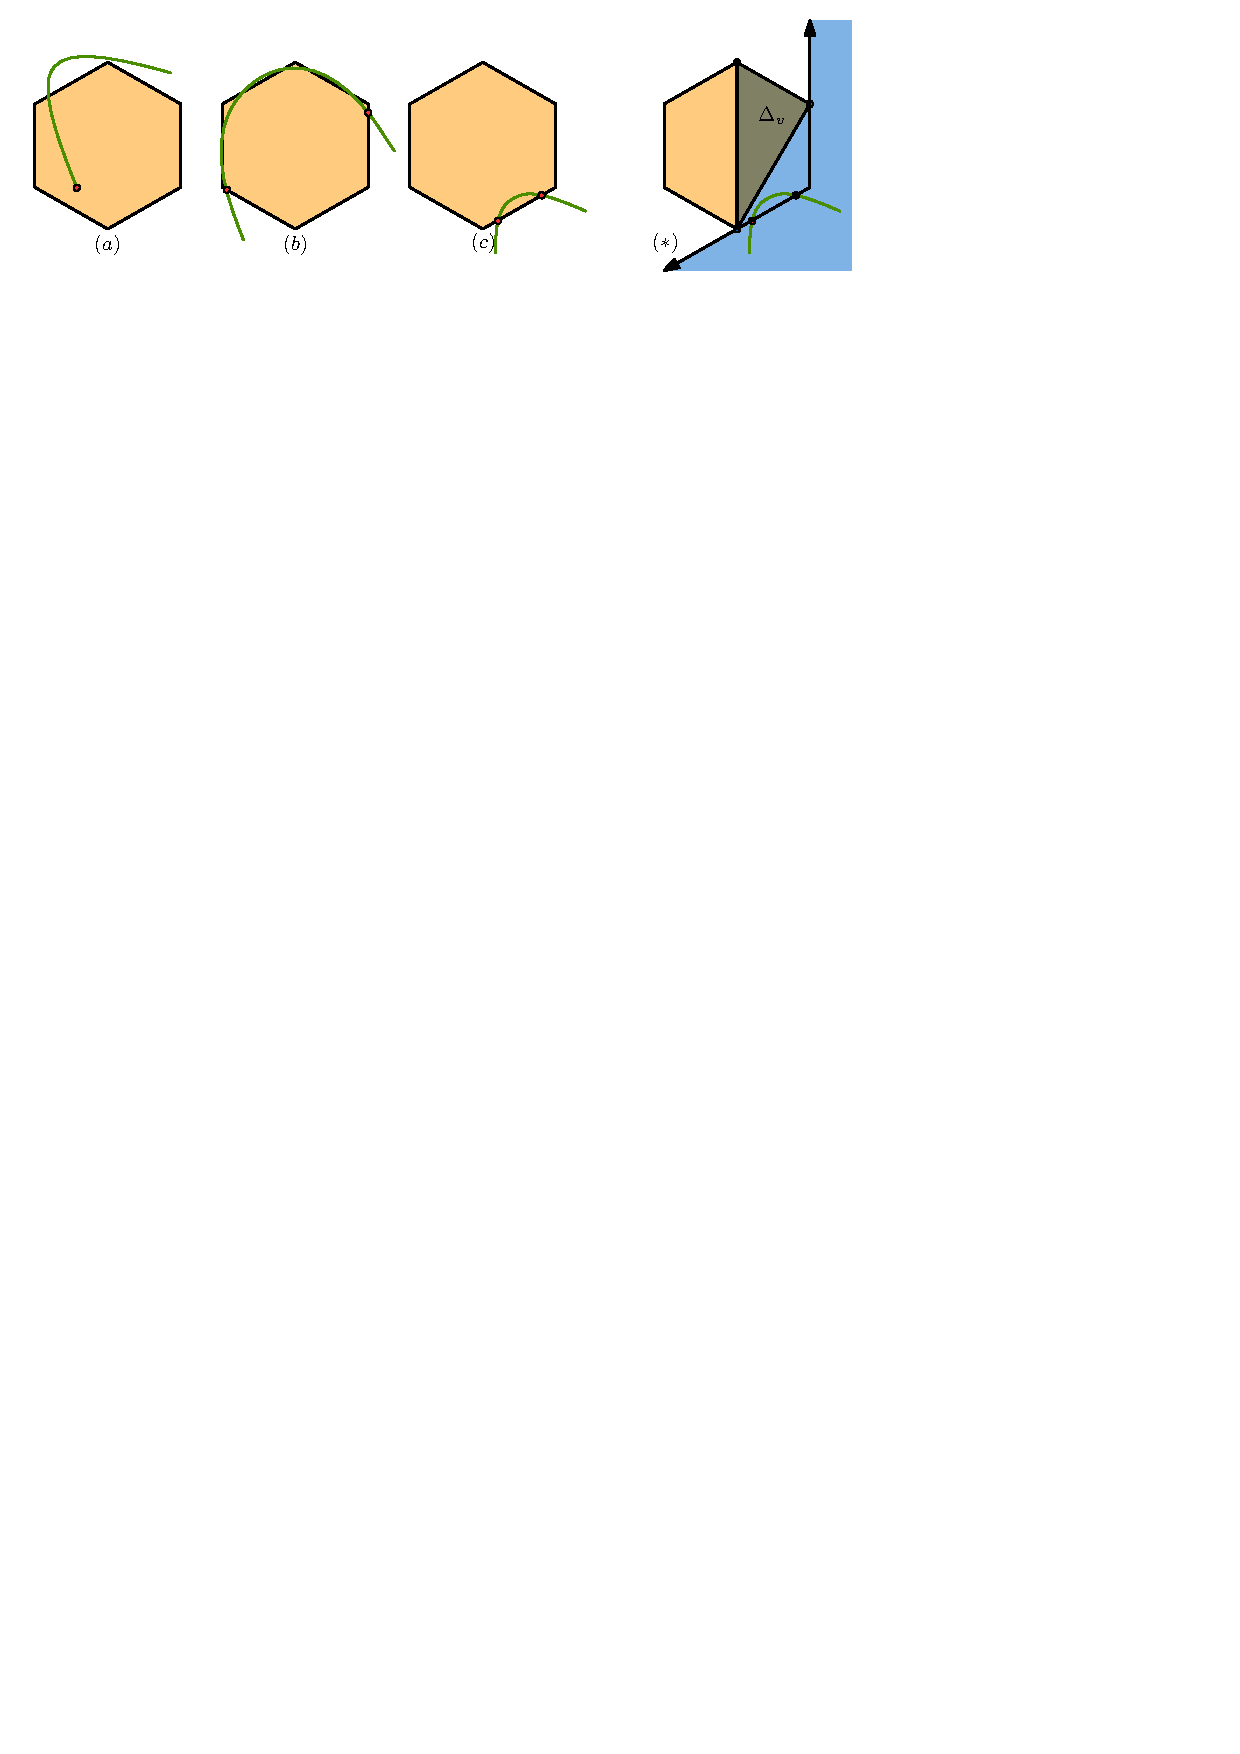
\includegraphics{../intersectionsearch}
    \caption{If $\gamma$ intersects $P_E$, then (a) an endpoint of $\gamma$ lies within $P_E$, or (b) $\gamma$ cuts off a vertex, or (c) $\gamma$ intersects only one edge of $E$ twice and has no endpoint in $P_E$ (we call this dipping).}
    \label{fig:intersectionsearch}
\end{figure}


\subparagraph{Intersection types (a) and (c).}
Chazelle \cite{FRANK} shows that you can preprocess $P_E$ using $\Theta(n)$ time and space, such that point location (and thus the detection of case (a)) can be done in $\Theta(\log n)$ time. To detect an intersection of case $(c)$, we first build a hierarchical triangulation of $P_E$ using $\mathcal{O}(n)$ space and $\mathcal{O}(n \log n)$ preprocessing time. Given $\gamma$, we recursively answer the intersection query as follows (Figure~\ref{fig:intersectionsearch} (*)): any node $v$ in this decomposition represents a sub-polygon $P'$ of $P_E$ and a triangle $\Delta_v$ which splits $P'$ in a left and right part. Consider the border of the right part $R = (e_1, e_2, \ldots, e_m)$. Note that if $\gamma$ does not intersect $\Delta_v$, then $\gamma$ can only dip an edge in $R$ if it is contained in the union of the half-spaces given by the lines through: (1) one edge of $\delta_v$ and (2) $e_1$ and $e_m$ (refer to the blue area in the figure). Given the node $v$ we do three things in constant time each: first we check if $\gamma$ intersects $\Delta_v$. If not then we check for both the left and right sub-polygon if $\gamma$ is contained in the specified area. If that is the case for both or neither sub-polygons then $\gamma$ can never dip an edge of $P_E$, else we recurse. It follows that we can detect case $(c)$ in $\mathcal{O}(\log n)$ time.

\subparagraph{Intersection type (b)}

We say that the curve $\Gamma$ of which $\gamma$ is a segment divides the plane into the interior and exterior. An edge $(x_1, x_2) \times (x_3, x_4) \in E$ is intersected by $\gamma$ with an intersection of type $(b)$ only if one endpoint lies in the interior and the other in the exterior. The points $(x,y)$ on the interior of $\Gamma$ are the $(x, y)$ for which $a_1 x^2 + a_2 x + a_3 xy + a_4 y + a_5 y^2 + a_6 \le 0$. This formulation gives a straightforward linearization and transforms the question if a point $\vec{x} = (x_1, x_2)$ lies on the interior of $\Gamma$ into a halfspace range query in $\mathbb{R}^5$. 

It follows \cite{chan2012optimal, chazelle1993cutting} that we can preprocess $E$ in $\mathcal{O}(S(5))$ and $\mathcal{O}(C(5))$ space and time, such that we can find for any curve segment $\gamma$ all the edges of $E$ which cross $\Gamma$ in $\mathcal{O}(Q(5))$ time represented as at most $\mathcal{O}(\log n)$ binary search trees $T_1 \ldots T_m$. Consider the clockwise ordering of the edges in such a tree $T_i$: the subset of these edges which are intersected by the segment $\gamma$ must be a connected chain in this order. Thus during preprocessing, we build for each subtree $T_i$ a binary search tree on the clockwise order on the edges in $T_i$ from which we can access this subset in $\mathcal{O}(\log n)$ time for each $T_i$. The time and space needed for solving case $(b)$ dominates the time and space needed for case $(a)$ and $(c)$ and we conclude:

\begin{theorem}
    We can preprocess a simple polygon $P_E$ in $\mathcal{O}(S(5) \log n)$ and $\mathcal{O}(C(5) \log n)$ space and time, such that for any degree-2 curve segment $\gamma$ we can find if there is an intersection between $\gamma$ and at least one edge in $E$ in $\mathcal{O}( Q(5) log^2 n)$ time. 
\end{theorem}

\section{Point-Line}


In this setting we have two entities $q$ and $r$ in a polygonal domain $P$ where $q$ is stationary whilst $r$ traverses a line segment. We consider three variants of this setting: one where $P$ is a simple polygon and $r$ is contained in $P$, one where $P$ is a simple polygon and one where $P$ is a polygonal domain. In every variant we are interested in preprocessing $P$ such that given $q$ and $r$, we can determine if there is a time where $q$ and $r$ are mutually visible in sub-linear time. For reasons that will become apparent later, we say that entity $r$ walks along the line $\rho := \{ x,y \mid  0 = a_1 x - a_2 - y \}$ from the point $s$ to the point $t$. Entity $q$ is stationary at the point $(a_3, a_4) \in P$ and $\rho$ is parametrized such that $q$ lies below $\rho$.

\begin{figure}[h]
    \centering
    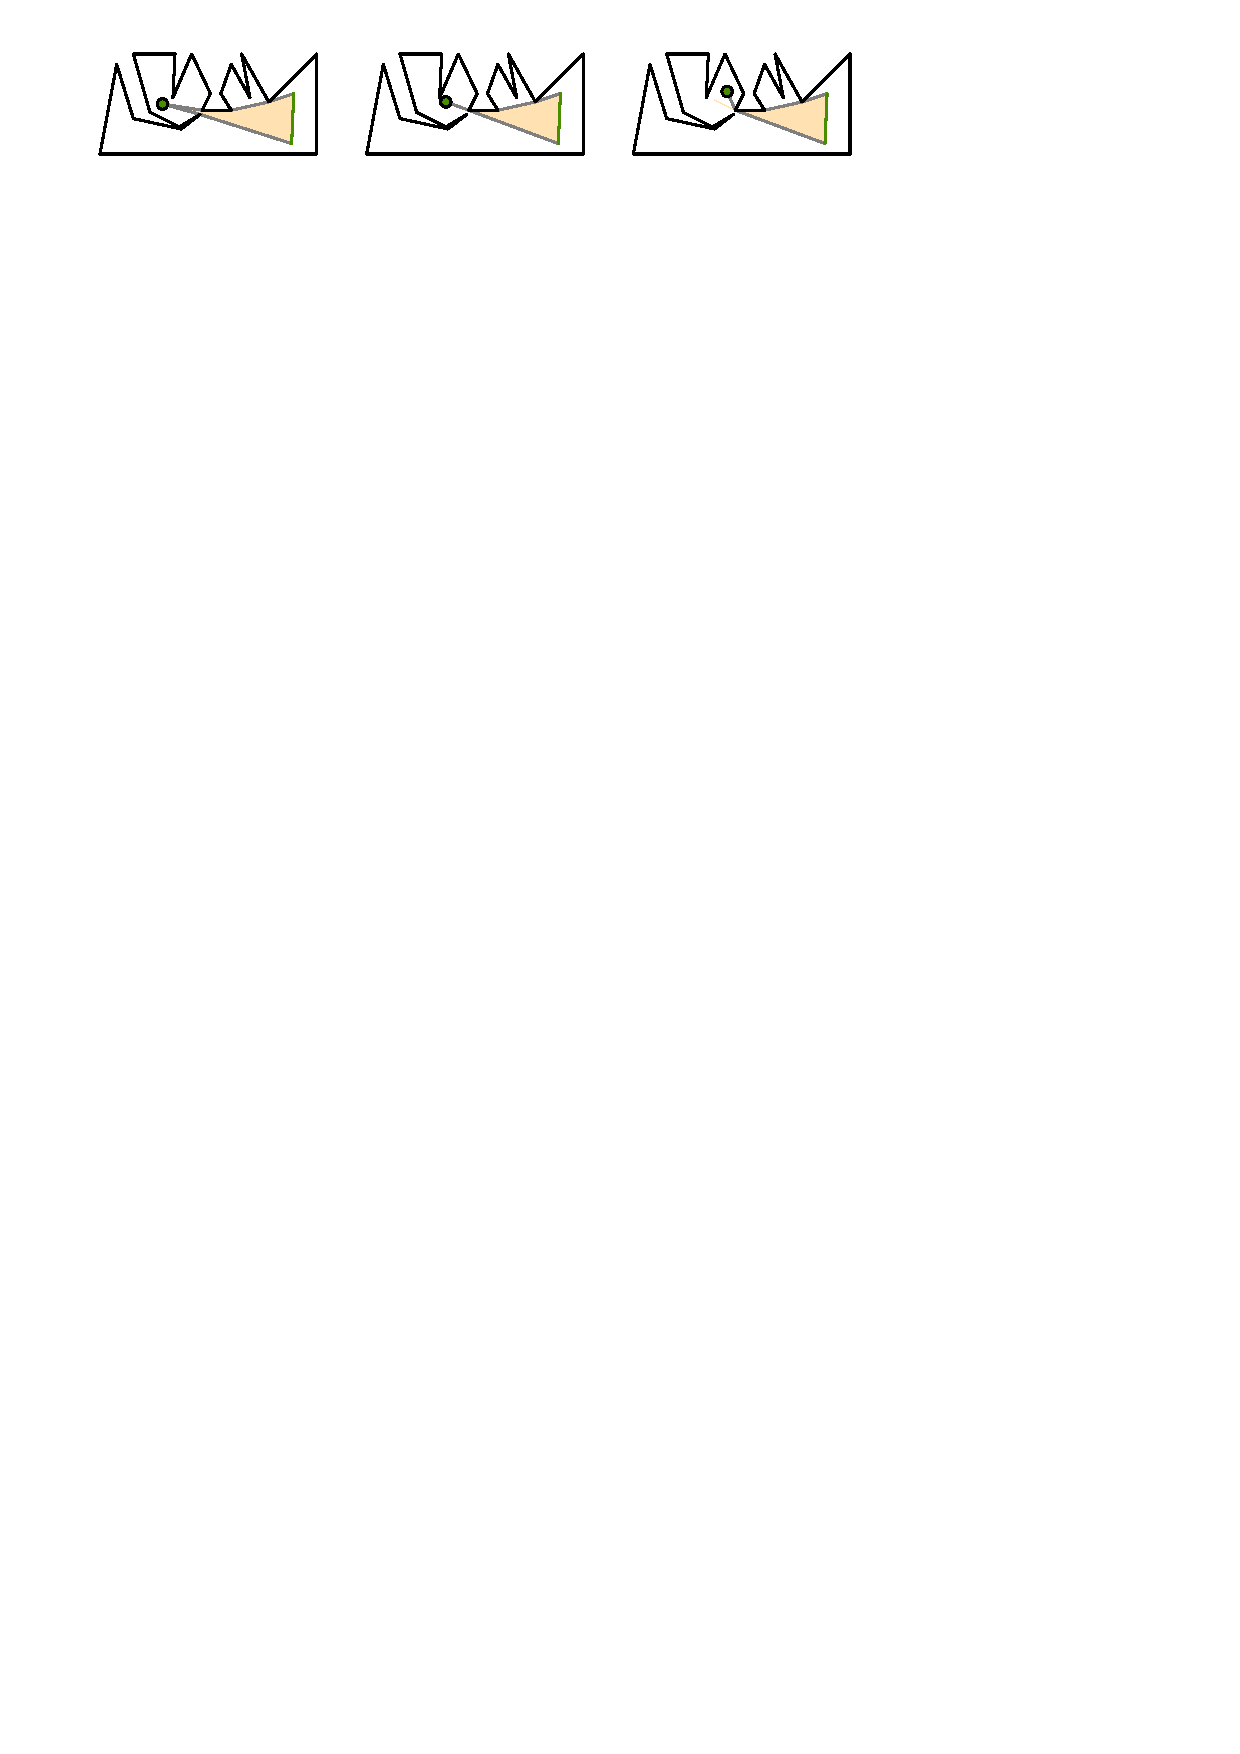
\includegraphics[]{../funnel}
    \caption{Three times a query pair $(q,r)$ in a simple polygon. In the middle case, the paths $\pi_1, \pi_2$ share their first line segment but there still is a point on $r$ which is visible from $q$.}
    \label{fig:funnel}
\end{figure}

\subparagraph{$P$ is a simple polygon and $r$ is contained in $P$.}
Consider the two shortest paths $\pi_1, \pi_2$ from $q$ to  each endpoint of $r$. Observe that if edges of $\pi_1$ and $\pi_2$ coincide, they coincide in a connected chain from $q$. Moreover (Figure~\ref{fig:funnel}) if more than one line segment of $\pi_1$ and $\pi_2$ coincide, then any shortest path from $q$ to a point on $r$ cannot be a single line segment. If no edges of $\pi_1$ and $\pi_2$ coincide then there is at least one point on $r$, whose shortest path to $q$ is a line segment. If exactly one line segment of $\pi_1$ coincides with a segment of $\pi_2$, then that segment must be connected to $q$ and if there is a line-of-sight between $q$ and $r$, it has to follow that line segment. This observation gives us an algorithm for the visibility query in this scenario: we simply build the shortest path data structure from Guibas and Hershberger which takes $\Theta(n)$ space, has $\mathcal{O}(n \log n)$ construction and $\Theta(\log n)$ query time. Given $q$ and $r$, we use this data structure to obtain $\pi_1$ and $\pi_2$ and we check whether the first and second edge coincides. If only the first edge coincides we trace its supporting line and check if we reach $r$ without intersecting $\pi_1$ or $\pi_2$ using their binary tree representation.

\begin{theorem}
We can preprocess a simple polygon $P$ in $\Theta(n)$ space and $\mathcal(n \log n)$ time. Such that for any query point $q$ and segment trajectory $r$ which is contained in $P$, we can determine if there is a point on $r$ that is visible from $q$ in $\mathcal{O}(\log n)$ time.
\end{theorem}




\subparagraph{$P$ is a simple polygon.}
If $r$ is able to move through edges of $P$ then answering the visibility query becomes significantly more complicated: $r$ could consist of linearly many sub-segments whose endpoints lie on the border of $P$. Inspecting each of these segments takes too much time. For any point $q \in P$, its visibility polygon $V_q$ is the union of all points which are visible from $q$. If $r$ intersects $V_q$, the point of intersection is a point on $r$ which is visible from $q$. It is possible to preprocess an explicit polygon $P'$ such that an intersection between $P'$ and a line segment can be determined in logarithmic time. However, so far no data structure exists that can return $V_q$ for any point $q$ in its explicit form.


We instead construct a three-level data structure. The base level is from Aronov \etal. Their data structure partitions $P$ into $\mathcal{O}(n^2)$ triangles, where for each triangle all points in that triangle have the same implicit visibility polygon, stored as a red-black tree on its edges. Each of these $\mathcal{O}(n^2)$ red-black trees could have linear size, so a naive implementation of the Aronov \etal data structure could take $\mathcal{O}(n^3)$ space. We first explain our data structure using this naive implementation. We then show that the red-black tree together with its secondary structures can be made partially persistent (just like the Aronov \etal data structure itself) which reduces the space requirement by a linear factor.

The implicit polygon $V_q$ could contain $\mathcal{O}(n)$ uncertain edges and depending on the location of $q$ the query segment $r$ may or may not intersect one (Figure~\ref{fig:twolevel}, middle). Consider the two rays from $q$ towards the start and end point of $r$ and denote the edges of $V_q$ hit by these rays as $e_1$ and $e_2$. If $r$ intersects $V_q$ then it must intersect an edge in the consecutive chain between $e_1$ and $e_2$. The second level of our data structure finds this chain. We assumed that every triangle of the partition of $P$ contained a unique red-black tree representing an implicit visibility polygon. Chazelle \etal \cite{chazelle1994ray}  created a data structure which can preprocess any simple polygon in $\mathcal{O}(n)$ space and $\mathcal{O}(n \log n)$ time, such that for any ray one can find the edge hit by the ray in$\mathcal{O}(\log n)$ query time. On top of each node in the red-black tree we build this ray shooting data structure. Ray shooting does not immediately work for any ray in $V_q$ since some edges are uncertain. However, it does work for rays originating from $q$ because each ray from $q$ per definition only stabs one edge from $V_q$.  We find $e_1$ and $e_2$ in the red black tree and with them $\mathcal{O}(\log n)$ subtrees that form our chain.

Consider a subtree $T$ returned by the second level. The root of this subtree represents a collection of $\mathcal{O}(n)$ certain and uncertain edges. Denote by $U$ the set of uncertain edges of $T$ and by $\bar{U}$ the certain edges. We build two separate data structures on top of $T$ that search for an intersection between $r$ and an edge in $\bar{U}$ or $U$ respectively. The data structure on $\bar{U}$ is the ray shooting data structure that we mentioned above. If a ray from the start of $r$ to end end of $r$ hits a certain edge, we know that we found a point on $r$ that can see $q$. The data structure on $U$ is an $8$-dimensional halfspace range search structure: 

\begin{lemma}
\label{lemma:uncertain_intersection}
For each edge $e \in U$, there is a unique 8-dimensional point, such that for each query pair $(q, r)$ there is a unique $8$-dimensional halfspace, such that $r$ intersects $e$ if and only if the point of $e$ is in that halfspace.
\end{lemma}



\begin{figure}[h]
    \centering
    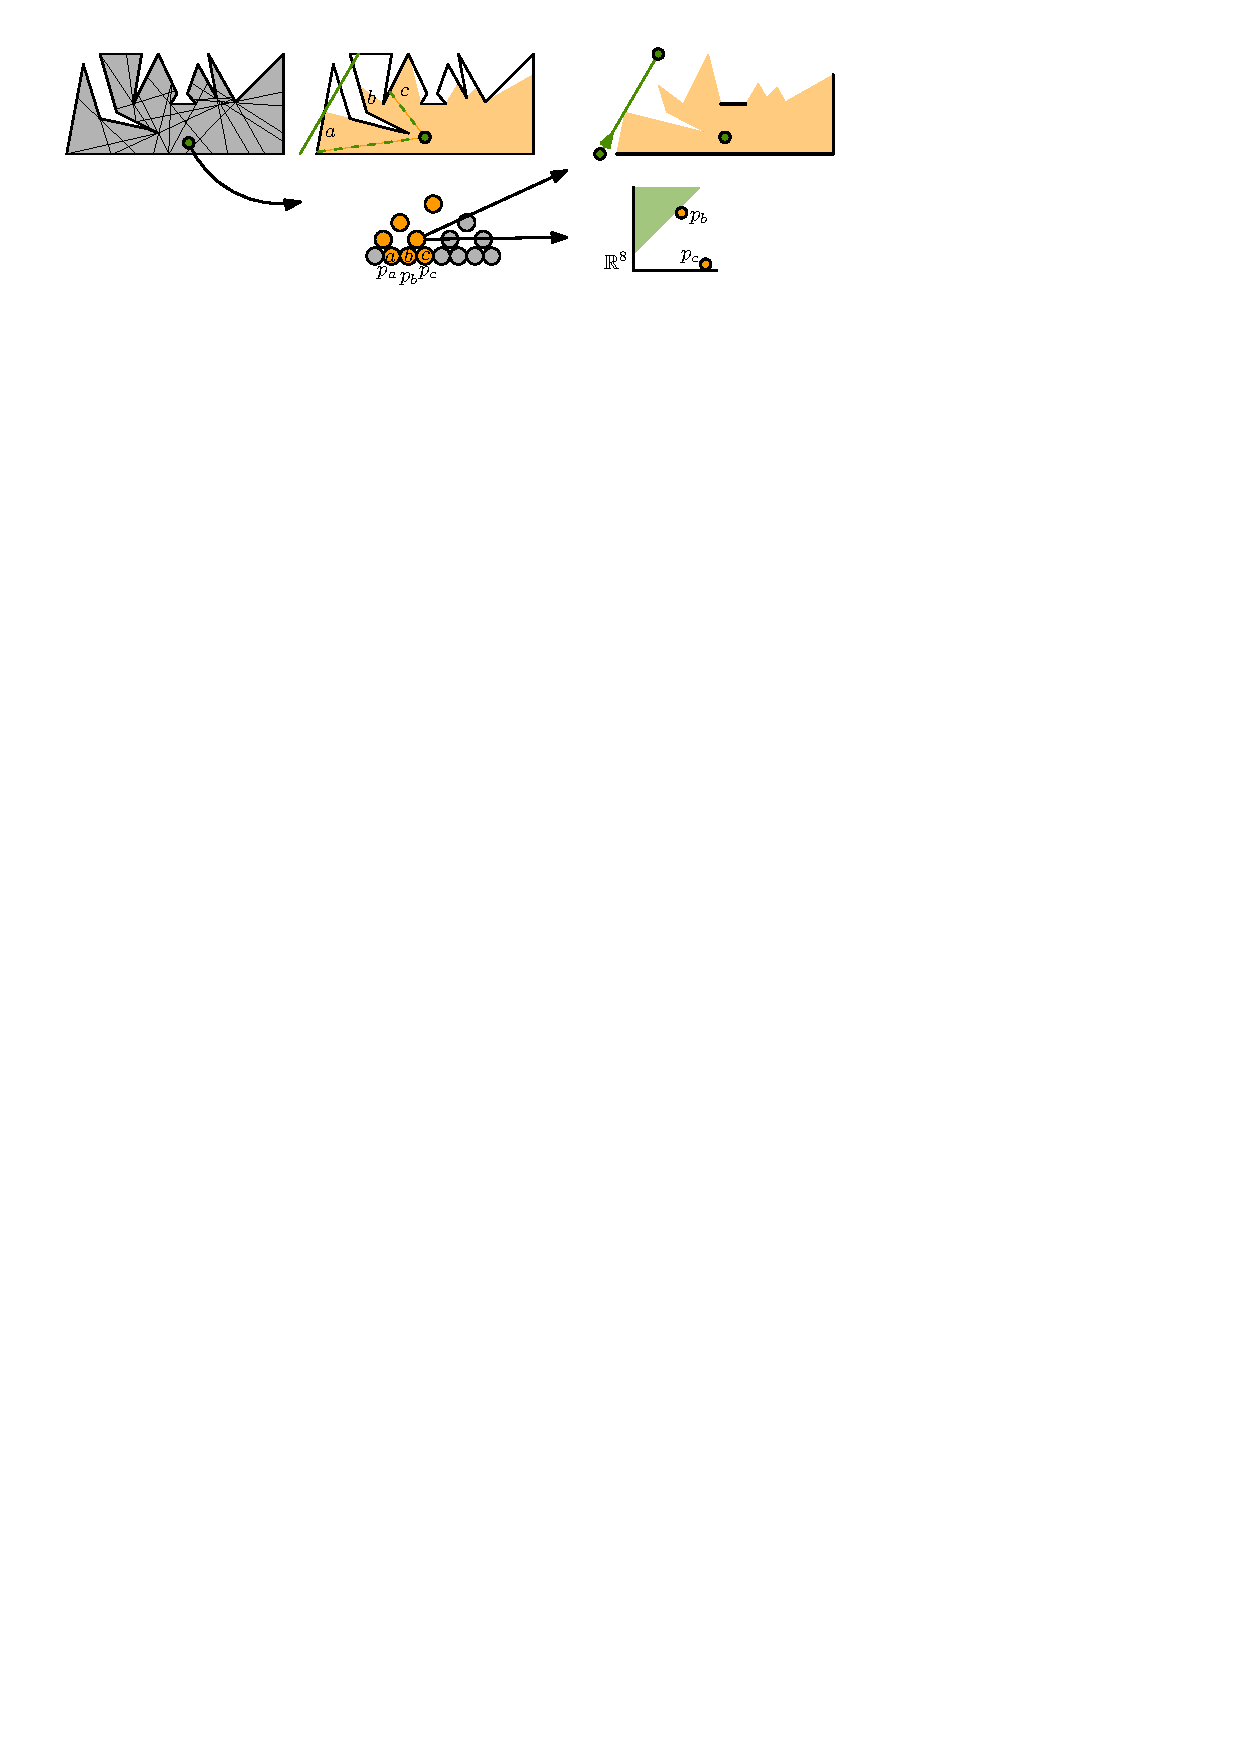
\includegraphics[]{../twolevel}
    \caption{ (left) A simple polygon split in $\mathcal{O}(n^2)$ triangles. For each triangle, there exists a red-black tree that represents a visibility polygon. (middle) Given $V_q$ and $r$, $r$ could intersect the explicit $V_q$ depending on the location of $q$. We shoot two rays from $q$ to $r$ and find their intersection with $V_q$ in the red-black tree. That gives us three leaves highlighted in orange. (right top) All the certain edges in this node are stored in a ray-shooting data structure, (right bottom) all the uncertain edges have 8-dimensional points that are stored in an $8$-dimensional partition tree.}
    \label{fig:twolevel}
\end{figure}


Our final data structure (Figure~\ref{fig:twolevel}) looks as follows: let $\Delta_q$ be a triangle in $P$ representing an implicit visibility polygon $V_q$. To each uncertain edge of $V_q$ we assign an $8$-dimensional point. $\Delta_q$ stores a red-black tree and for each node in this tree we do two things: (1) we identify the uncertain edges in this node and we build an $8$-dimensional partition tree on their corresponding points, (2) we identify the certain edges and build a ray shooting data structure on these points.
$8$-dimensional partition trees on $m$ points take $\mathcal{O}(S(8))$ space and can be constructed in $\mathcal{O}(C(8))$ time and this dominates the time and space requirement for the ray shooting data structure. Each edge of $V_q$ occurs in at most $\mathcal{O}(\log n)$ nodes and thus two-level data structure in $\Delta_q$ takes up at most $\mathcal{O}(S(8) \log n)$ space per triangle $\Delta_q$.

At query time we first find the triangle $\Delta_q$ containing $q$ in $\mathcal{O}(\log^2 n)$ time. The secondary layer identifies at most $\mathcal{O}(\log n)$ subtrees in $\Delta_q$ which together for the relevant portion of the border of $V_q$. Given $r$ and $q$, we compute an $8$-dimensional halfspace query range in constant time and we query the partition trees of each of these $\mathcal{O}(\log n)$ trees in $\mathcal{O}(S(8))$ time which dominates the earlier time used to find $\Delta_q$. There is an intersection between $r$ and an uncertain edge of $V_q$ if and only if at least one of these query ranges is non-empty.  Thus we can conclude:

\begin{theorem}
We can preprocess a simple polygon $P$ in $\mathcal{O}(S(8) n^2 \log n)$ space and $\mathcal{O}(C(8) n^2 \log n)$ time. Such that for any query point $q$ and segment trajectory $r$, we can determine if there is a point on $r$ that is visible from $q$ in $\mathcal{O}(Q(8) \log n)$ time.
\end{theorem}




\subparagraph{Polygonal domains, persistence with transient updates.}

Frank proves that $n^2$ is really $n^2$ and not $n^3$. Moreover, Vegter and Pol-whatever exist for polygonal domains.


\section{Line-Line}
\label{sec:lineline}


In this setting we have two entities $q$ and $r$ in a polygonal domain $P$ which both traverse a line segment, possibly at different (constant) speeds, during the time interval $t \in [0,1]$. We consider three variants of this setting: one where $P$ is a simple polygon and $q$ and $r$ are contained in $P$, one where $P$ is a simple polygon and one where $P$ is a polygonal domain. In every variant we are interested in preprocessing $P$ such that given $q$ and $r$, we can determine if there is a time $t^* \in [0,1]$ where $q$ and $r$ are mutually visible in sub-linear time. For reasons that will become apparent later, we say that entity $q$ walks from the point $(a_1, a_2)$ to $(a_1 + a_3, a_2 + a_4)$ and entity $r$ walks from the point $(a_5, a_6)$ to $(a_5 + a_7, a_6 + a_8)$. Note that the respective speed of $q$ and $r$ is $\lVert (a_3, a_4) \rVert$ and $\lVert (a_7, a_8) \rVert$ respectively.

\subparagraph{P is a simple polygon and $r$ and $q$ are contained in $P$.}
The hourglass $H(q, r)$ is the union of all the shortest paths between $q$ and $r$. 
Recall that $H(q,r)$ is a polygon bound by the shortest paths between the endpoints of $q$ and $r$ and $q$ and $r$ itself. There is a special case for $H(q,r)$ which is when either $q$ or $r$ does not lie on the polygonal boundary of $H(q,r)$. We call this case a \emph{funnel} (Figure~\ref{fig:visibilityglass} (a)). If $H(q,r)$ is a funnel, then visibility between $q$ and $r$ can be checked in the same way as in the previous section.

The hourglass $H(q, r)$ usually contains many shortest paths which are not line segments. A line-of-sight is a shortest path which is a single line segment and hence $H(q,r)$ contains too much information. We define the \emph{visibility glass} $L(q,r)$ as the collection of line segments between $q$ and $r$ that are contained in $P$. $L(q,r)$ is a subset of $H(q,r)$ and could be empty. Observe that if $L(q,r)$ is empty then $q$ is never visible from $r$, but the converse is not neccecarily true (Figure~\ref{fig:nointersect}). However the two entities are mutually visible at time $t$ if and only if the line segment between them is contained within $L(q,r)$. For any query segments $q$ and $r$, we can obtain $L(q,r)$ using the following lemma from Chazelle and Guibas:

\begin{lemma}[Lemma 2.1 from \cite{Chazelle1989}]
For any two line segments $q, r \in P$, there exist two line segments $q' \subset q, r' \subset r$ such that $V(q, r) = H(q', r')$. Moreover, $q'$ and $r'$ are induced by the bitangents of the polygon $H(q, r)$.
\end{lemma}

If $H(q,r)$ is not a funnel then $H(q,r)$ is bouned by $q, r$ and two semi-convex subchains which we refer to as the upper and lower chain which end in upper and lower endpoints of $q$ and $r$. Consider the shortest path $\pi$ from the upper point of $q$ to the lower point of $r$. $\pi$ partially coincides with the upper and lower chain, and its two coinciding paths are joined by a single line segment. The extension of this line segment is the bitangent of $H(q,r)$~\cite{FRANK}. Since the upper and lower chain are convex chains, all segments on the lower chain start and end in a clockwise rotation and segments on the upper chain start and end with a counter-clockwise rotation. The bitangent segment is the only segment on $\pi$ that starts with a clockwise and ends with a counter-clockwise rotation. 


\begin{figure}[h]
    \centering
    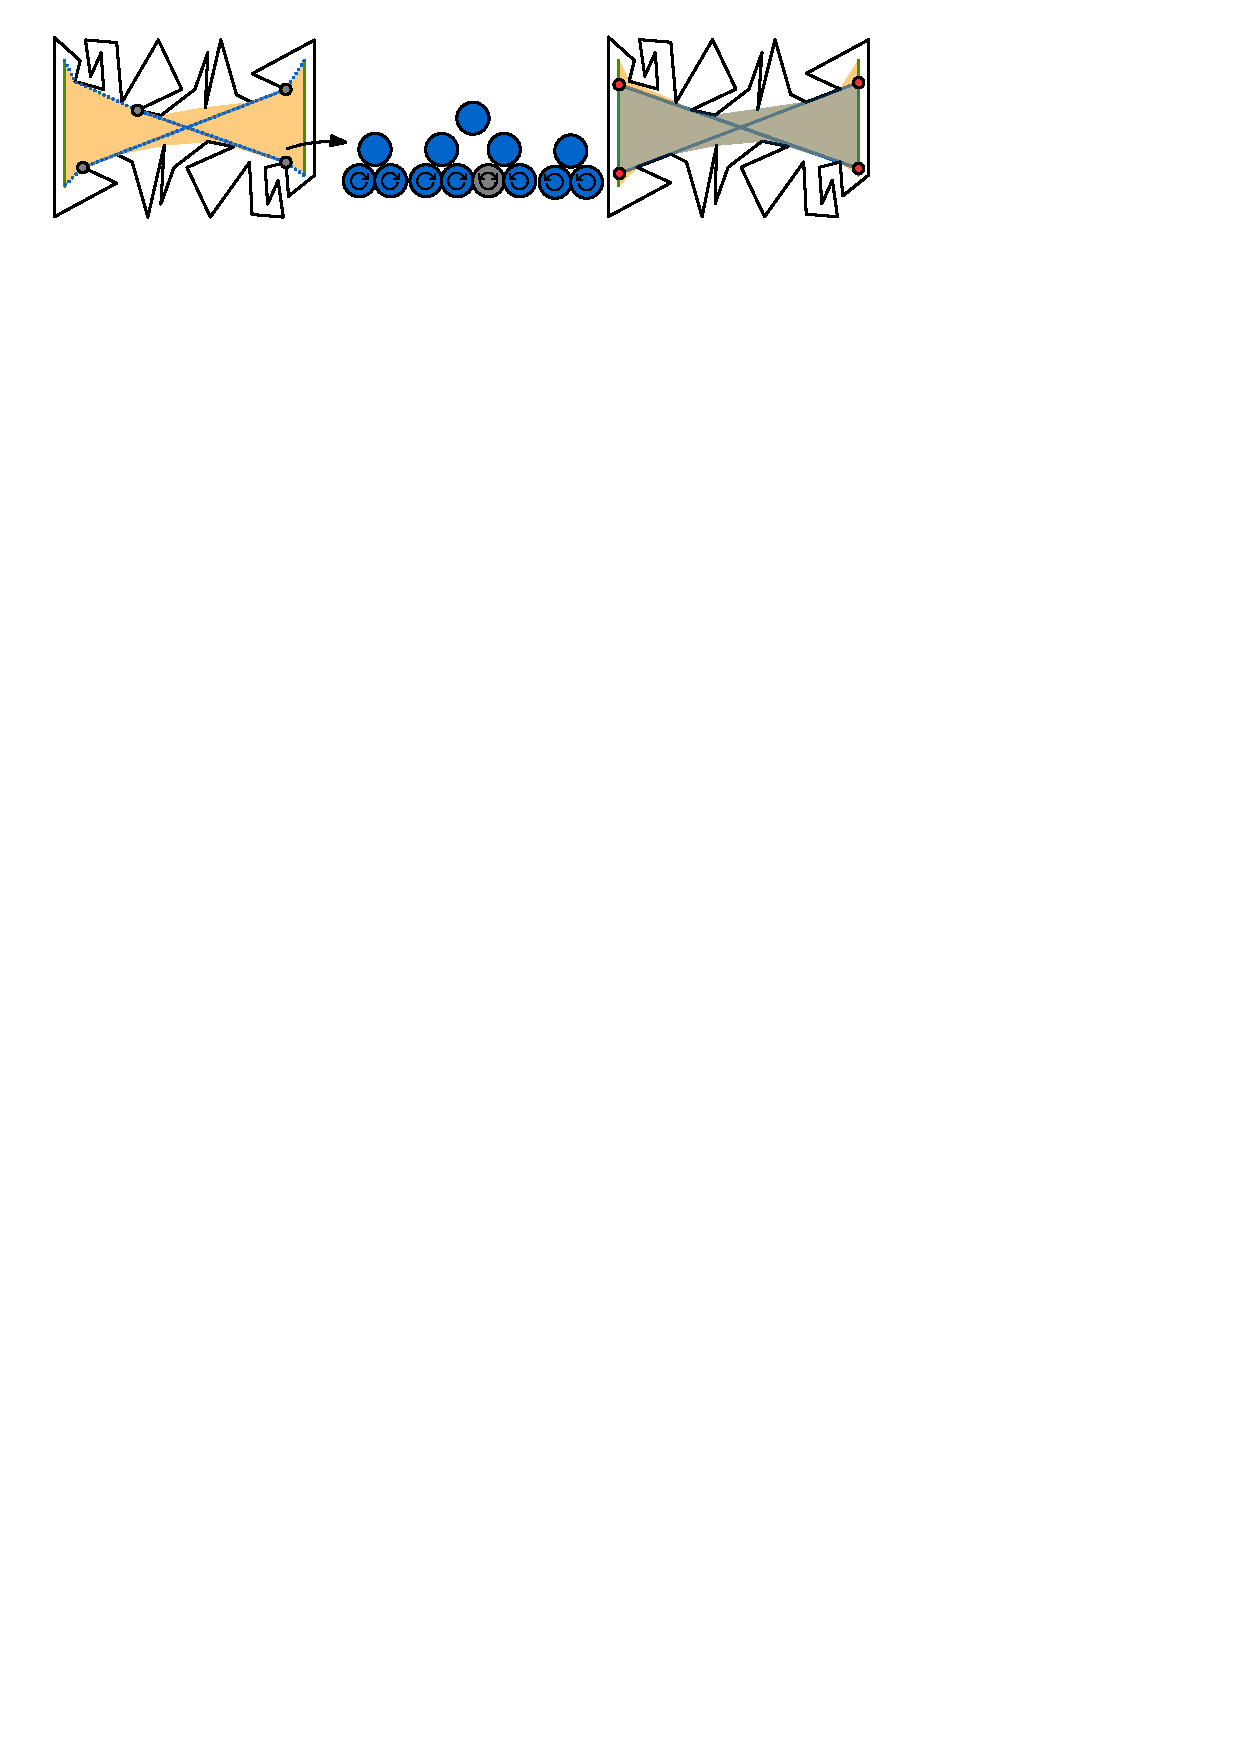
\includegraphics[]{../visibilityglass}
    \caption{(left) a simple polygon containing $q$ and $r$. $H(q,r)$ is shown in orange. The shortest paths between endpoints are shown in dotted blue and the bitangents are underlined in grey. (middle) we obtain each dotted path as a collection of binary search trees, where only the bitangent starts in clockwise and ends in counterclockwise rotation. (right) using the bitangents, we identify the endpoints of $q'$ and $r'$ and obtain $L(q,r)$ in blue. }
    \label{fig:visibilityglass}
\end{figure}

Using this information, we can obtain an implicit representation of $L(q,r)$ using the data structure $\mathcal{D}$ from Guibas and Hershberger (Refer to Figure~\ref{fig:visibilityglass}). Given $q$ and $r$, we can obtain the border of $H(q,r)$ as a set of $\mathcal{O}(\log n)$ concatenated persistent red-black trees. We can binary search these trees to detect if $H(q,r)$ is a funnel. If $H(q,r)$ is not a funnel, we can find the two bitangents of $H(q,r)$ as follows: we query $\mathcal{D}$ for the shortest path between the upper endpoint of $q$ and lower endpoint of $r$ and obtain this path as a set of $\mathcal{O}(\log n)$ red-black trees. We perform a binary search on these trees to locate the bitangent segment that starts with a clockwise and ends with a counter-clockwise rotation. We perform an identical procedure to identify the second bitangent.
These two bitangents bound the segments $q'$ an $r'$. We query $\mathcal{D}$ one more time with these two segments to obtain $H(q', r')$ and with it the visibility glass $L(q,r)$ in its implicit representation. Each query in $\mathcal{D}$ takes $\mathcal{O}(\log n)$ time and so does our binary search thus we conclude:

\begin{lemma}
\label{lemma:visibilityquery}
  The Guibas and Hershberger data structure can for any segment $q,r$ contained in $P$ obtain the implicit representation of $L(q,r)$ in $\mathcal{O}(\log n)$ time.
\end{lemma}

 
Given $L(q,r)$, we want to test if there is ever a time $t^*$ where the segment between the two entities lies in $L(q,r)$. (partitions visibility glass in two halves) Consider the set of lines through $L(q,r)$. \ivor{FRANK IS THIS TRUE} showed that a line segment between $q$ and $r$ coincides with a line segment in $L(q,r)$ if and only if their extended lines coincide. Chazelle and Guibas \cite{Chazelle1989} note, that if we dualise the collection of all lines through $L(q,r)$ then we obtain a convex polygon denoted by $\Lambda(q,r)$ of linear complexity. The line through the two entities coincides with a line in $L(q,r)$ if and only if its dualized point lies in $\Lambda(q,r)$. To detect if such a point exists, we use the following Lemma:

\begin{lemma}
\label{lemma:hyperbola}
  The continuous dualization of the line through the two entities, traces a hyperbolic segment $\gamma(t)$ for $t \in [0,1]$ with five degrees of freedom.
\end{lemma}

At this point, we have transformed the visibility query in the primal to an intersection query between a convex polygon and a hyperbolic segment in the dual and we implore our data structure from Section~\ref{sec:intersectionsearch}. In its general form, this data structure transforms an intersection query between a hyperbolic segment into a halfspace emptyness query in $\mathbb{R}^5$. Our query hyperbola has one fewer degrees of freedom than a general hyperbola which immediately makes it a halfspace emptyness query in $\mathbb{R}^4$ instead (refer to Equation~\ref{eq:hyperbola}).


\begin{figure}[h]
    \centering
    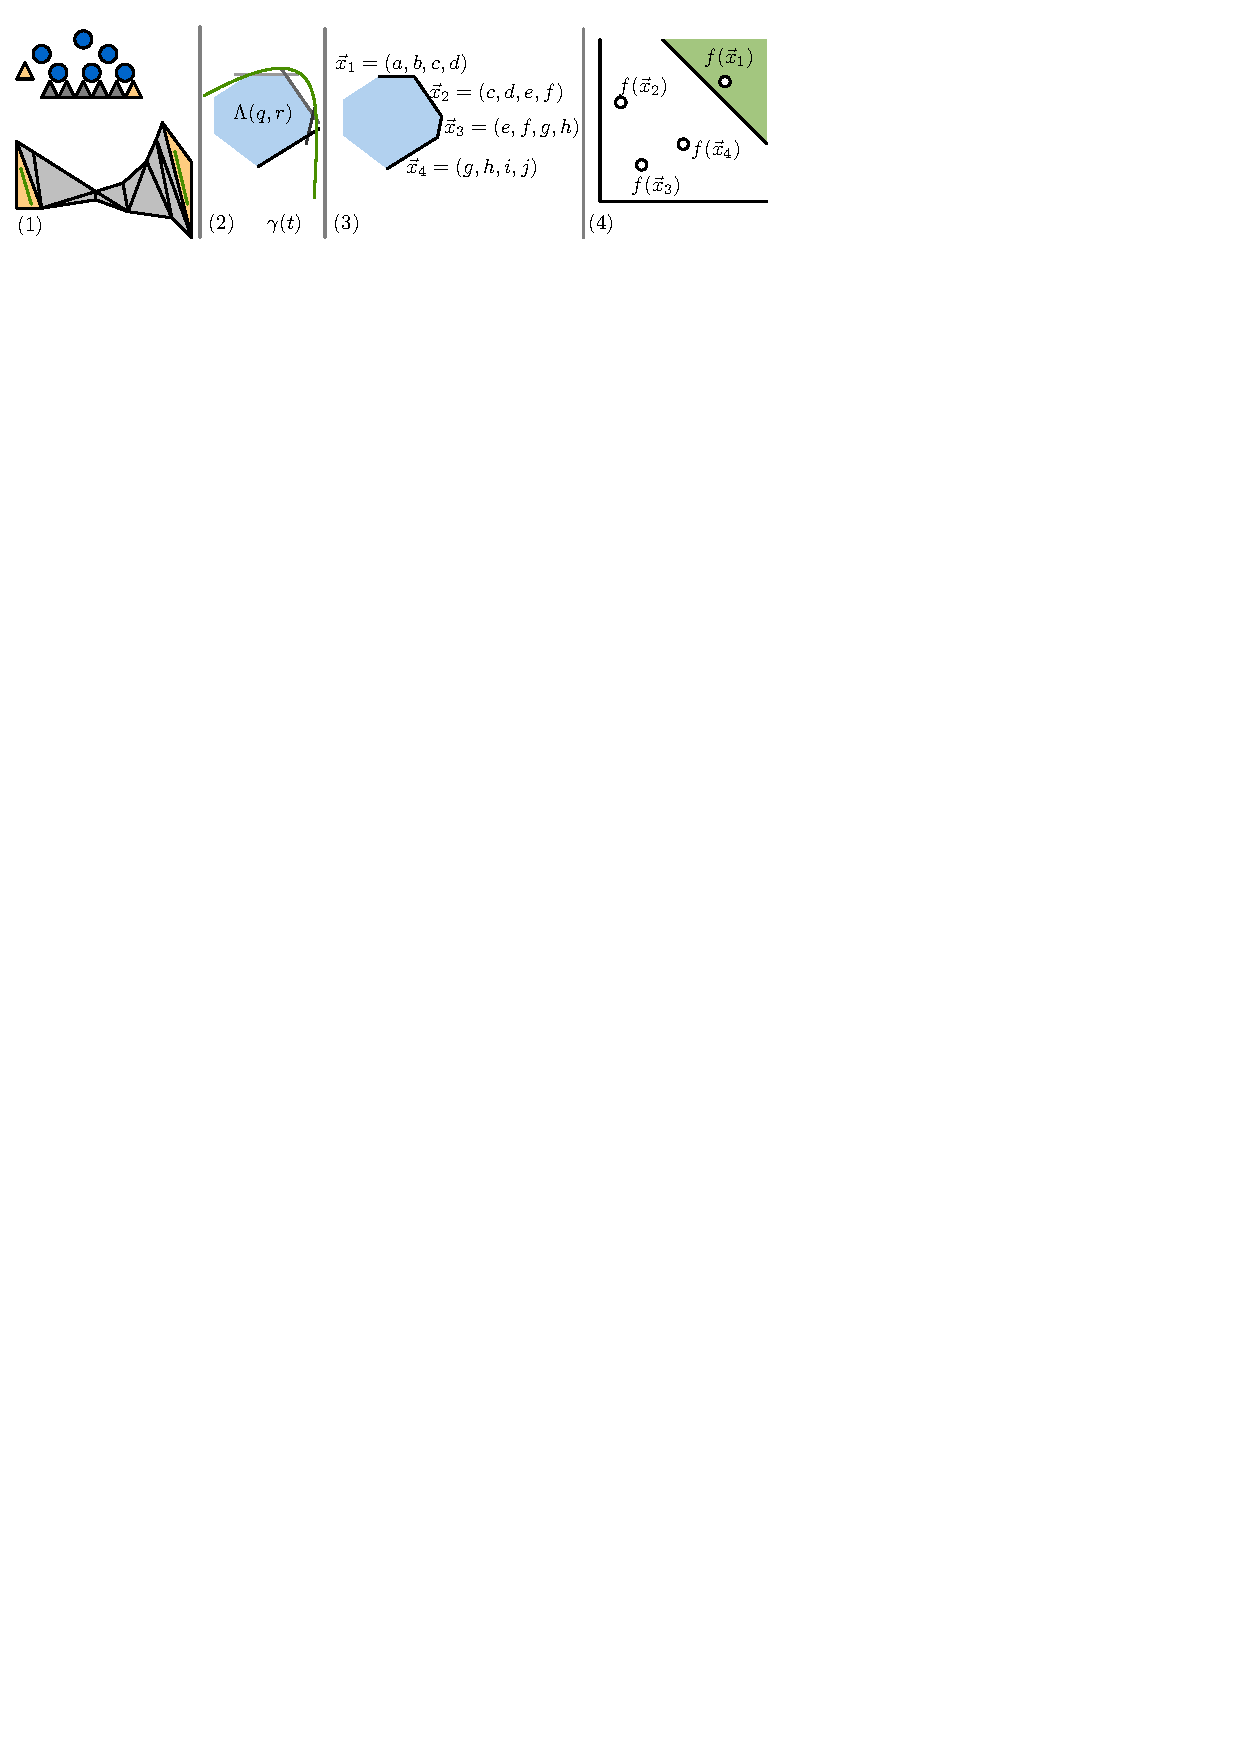
\includegraphics[]{../panel}
    \caption{(1) The base level of our data structure is the Guibas and hershberger hierarchical triangulation. (2) Given $q$ and $r$, we compute $\Lambda(q,r)$ which is the dual of the visibility glass between $q$ and $r$ and the degree-2 query curve $\gamma(t)$. (3) We store the parameters of each edge of $\Lambda(q,r)$ (4) Each parameter vector gets mapped to a point in $\mathbb{R}^4$ and the query curve gets mapped to a 4-dimensional halfspace. There is visibility between $q$ and $r$ if and only if this halfspace is non-empty.}
    \label{fig:panel}
\end{figure}


Our final data structure (refer to Figure~\ref{fig:panel}) is a two-level data structure with some interesting technicalities. The base data structure is the hierarchical decomposition $\mathcal{D}$ of $P$. The leaves of this tree represent a triangle in the triangulation of $P$ and every node in the tree stores the dual of constantly many hourglasses (which may be an unbounded region), represented as a red-black tree on its edges. Every vertex of $P$ in the primal, is contained in at most $\mathcal{O}(\log n)$ of these pre-stored hourglasses \cite{guibas1989optimal} so a naive implementation of this data structure would take $\mathcal{O}(n \log n)$ space. For ease of exposition, we first explain our data structure using the naive implementation. 

Every node of $\mathcal{D}$ represents a collection of line segments and possibly two halflines and each line segment has a unique representative point in $\mathbb{R}^4$. In the second level of our data structure we store the representative points in the two-level partition tree from Section~\ref{sec:intersectionsearch}. This data structure can store $m$ points in $m \log m$ space. Thus, the final data structure uses $\mathcal{O}(n log^2 n)$ space.

\subparagraph{Querying.}
When we get a query consisting of the line-segments
representing the trajectories of $r$ and $q$, we have to decide if there exists
a time $t^*$ at which $r$ and $q$ are mutually visible. Using Lemma~\ref{lemma:visibilityquery} we obtain the implicit representation of the visibility glass $L(q,r)$ in $\mathcal{O}(\log n)$ time. Recall that $L(q,r)$ is the concatenation of $\mathcal{O}(\log n)$ hourglasses: that is $L(q,r)$ is a collection of $\mathcal{O}(\log n)$ inward-convex chains $C_0 \ldots C_m$ (which are stored in a subtree of a red-black tree), each joined by an outer tangent $\tau_1 \ldots \tau_{m}$. Refer to Figure~\ref{fig:chain} for an example. Consider the dual $\Lambda(q,r)$ of the lines supporting $L(q,r)$. This convex polygon is a concatenation of the dual of each inward-convex chain in $C_1 \ldots C_m$ where each two chains $C_{i-1}, C_{i}$ are joined by a vertex which is the dual of $\tau_i$. 



\begin{figure}[h]
    \centering
    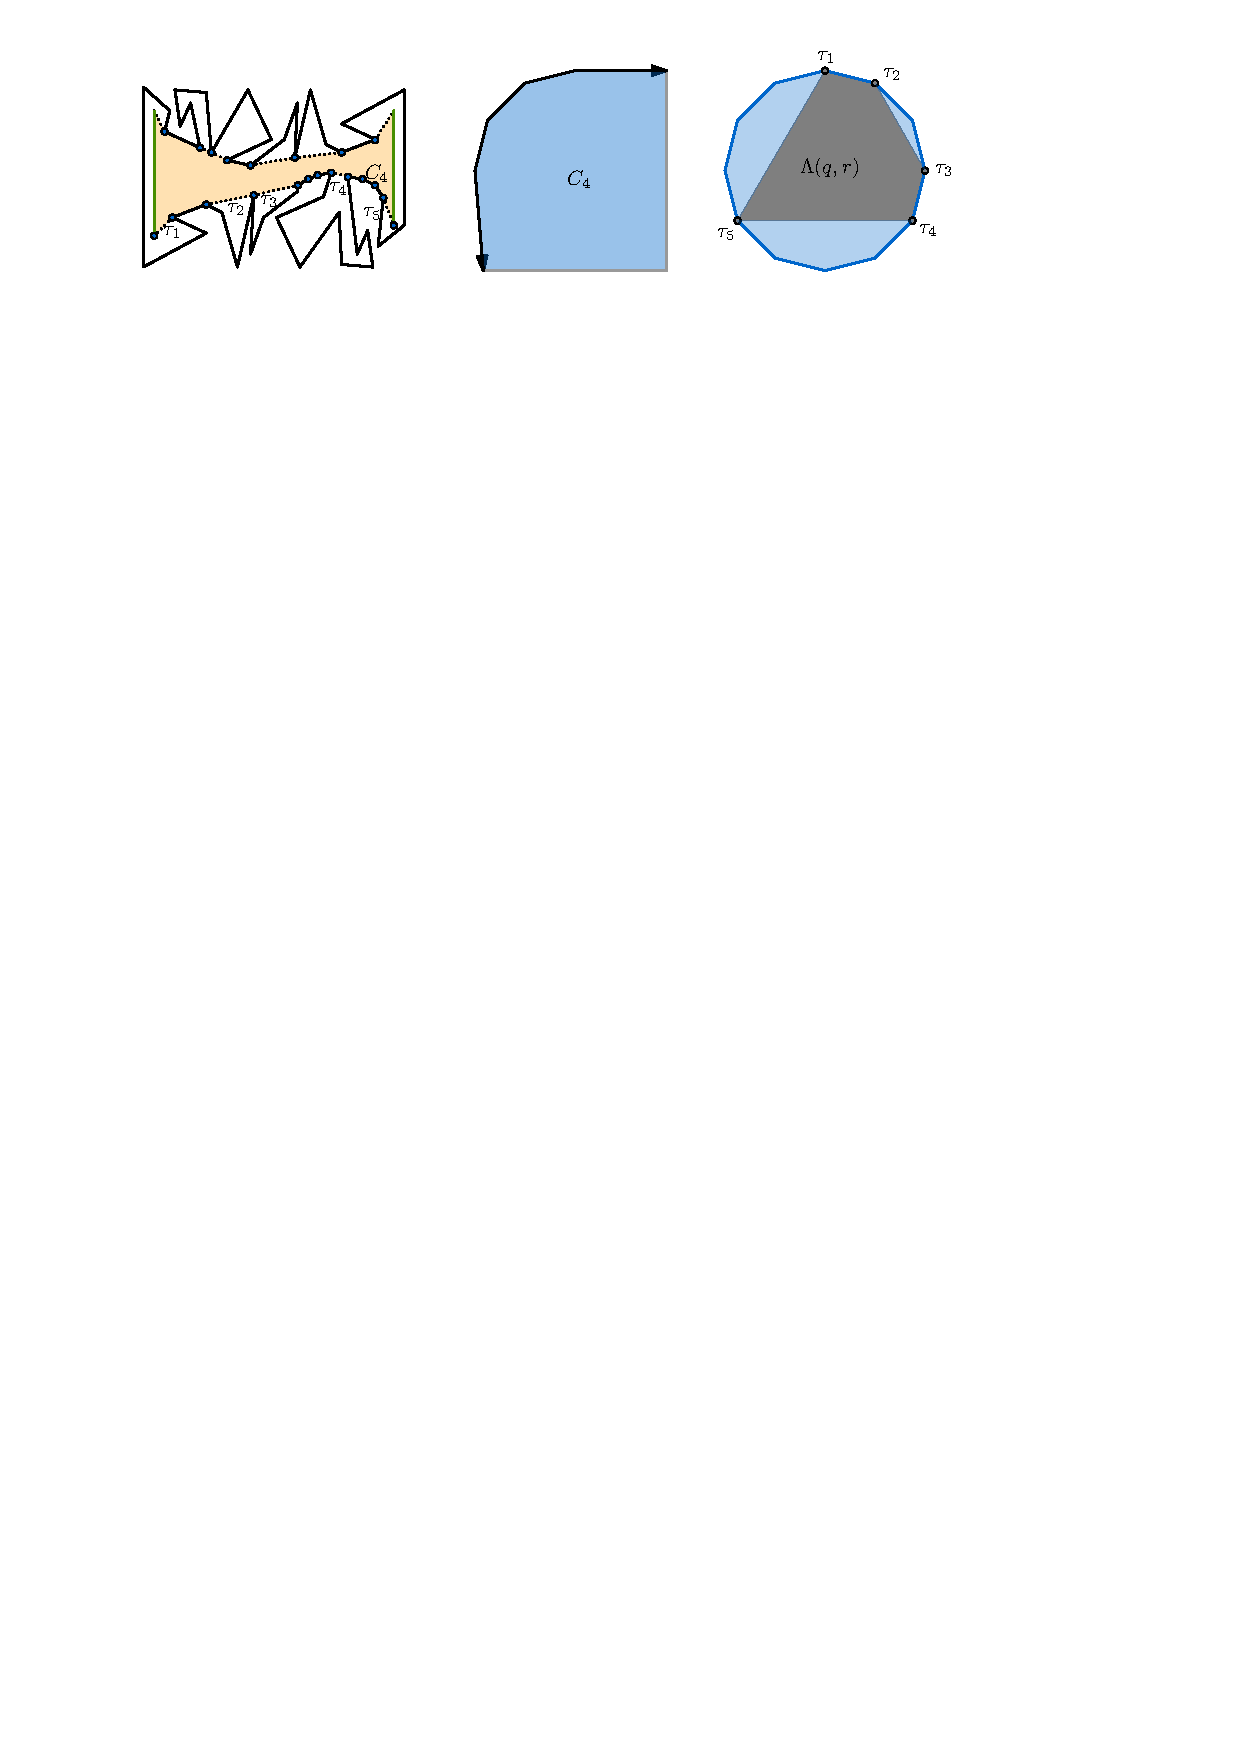
\includegraphics[]{../chain}
    \caption{(left) An hourglass between $q$ and $r$ in orange. The shortest path from the bottom of $q$ to the bottom of $r$ consists of five chains which coincide $P$ which are joined by outer tangents in dotted lines. We labelled the lower outer tangents $\tau_1 \ldots \tau_5$. (middle) An example of an area bound by the dualized chain $C_4$. (right) A simplified version of $\Lambda(q,r)$. Note that outer tangents could become vertices of $\Lambda(q,r)$.}
    \label{fig:chain}
\end{figure}


At this point, we would like to immediately search for an intersection between $\Lambda(q,r)$ and the query curve $\gamma(t)$, however a slight technicality appears. Consider the dualization of an inward-convex chain $C_i$ with respect to the polygon $\Lambda(q,r)$. $\Lambda(q,r)$ contains a subset of this chain, which is cut off by two outer-tangents which were not known before query time. These cut-off points were constructed during the Guibas and Hershberger query, so we can remember a pointer to each of the $\mathcal{O}(\log n)$ cut-off points induced by the outer-tangents. The result is, that the border of $\Lambda(q,r)$ is represented by at most $\mathcal{O}(\log n)$ red-black trees, which are bound by $\mathcal{O}(\log n)$ nodes induced by the outer tangents. The leaves of these trees are fixed vertices in $P$ (and therefore fixed edges in $\Lambda(q,r)$) and in the dual these fixed edges are joined by at most $\mathcal{O}(\log n)$ edges which we discover at query time.

Being aware of this technicality, we proceed as follows: we manually check if any of the $\mathcal{O}(\log n)$ uncertain edges intersect our query curve segment. If not, we have $\log n$ pre-stored trees where each tree represents a chain bordering $\Lambda(q,r)$. Recall that in Section~\ref{sec:intersectionsearch} we observed that a degee-2 curve segment can intersect a polygon in 3 cases labelled (a), (b) and (c). The argument for cases (b) and (c) still holds, but any subtree tree $T$ found by the base level of our data structure bounds a convex area which is larger than its portion on $\Lambda(q,r)$. However, observe the following: suppose an endpoint of the query segment lies within $\Lambda(q,r)$, in our application this means that either the two start points of $q$ and $r$, or the two end points of $q$ and $r$ can see one another. Checking if these two points are visible in the primal, can easily be done in logarithmic time. It follows that we can test for an intersection between our query curve segment and $\Lambda(q,r)$ in $\mathcal{O}(n^{3/4 + \varepsilon})$ time.

\begin{theorem}
    We can preprocess a simple polygon $P$ in $\mathcal{O}(n^{1 + \varepsilon} \log n )$ space and $\mathcal{O}(n^{1 + \varepsilon} \log^3 n)$ time. Such that for two query segment trajectories $q$ and $r$ contained in $P$, we can determine if there is a point on $r$ that is visible from $q$ in $\mathcal{O}(n^{\frac{3}{4} + \varepsilon} \log n)$ time.
\end{theorem}




\newpage
\bibliographystyle{abbrv}
\bibliography{../bib}



\newpage
\appendix

\section{Without Preprocessing}
We now consider the no-preprocessing version of detecting visibility between two trajectories. We will show that in the most general version of the problem, where the obstacles consist of $n$ arbitrary line segments, visibility can be checked in $O(n)$, which is obviously optimal.

Given two moving points $q(t)$ and $r(t)$ for $t \in [0, 1]$ and an obstacle segment $s$ we say visibility is obstructed at $t$ if $(q(t), r(t))$ intersects $s$ and unobstructed otherwise. For a fixed $q$ and $r$, a given segment $s$ partitions the interval $[0, 1]$ into up to $2$ obstructed and up to $3$ unobstructed regions. Let $U$ be the union of all the obstructed regions induced by every edge $e \in E$. If $U = [0,1]$ then at every time there is an obstacle blocking visibility between $q(t)$ and $r(t)$; if not, then there is a time $t$ at which they are mutually visible.

Thus our problem reduces to the following: given a set of $n$ intervals in $[0,1]$, determine if the union of the intervals is equal to $[0,1]$.

We start by allocating an array of length $n$, where each element $i$ corresponds to the interval $(\frac{i}{n}, \frac{i+1}{n})$ and setting each interval to uncovered. We then read the edg


\section{Prior Work/Lit Review}
\subsection{Visibility}
\subsection{Trajectories}

\section{Semi-algebraic range searching}
\label{appx:rangesearch}


\begin{figure}[h]
    \centering
    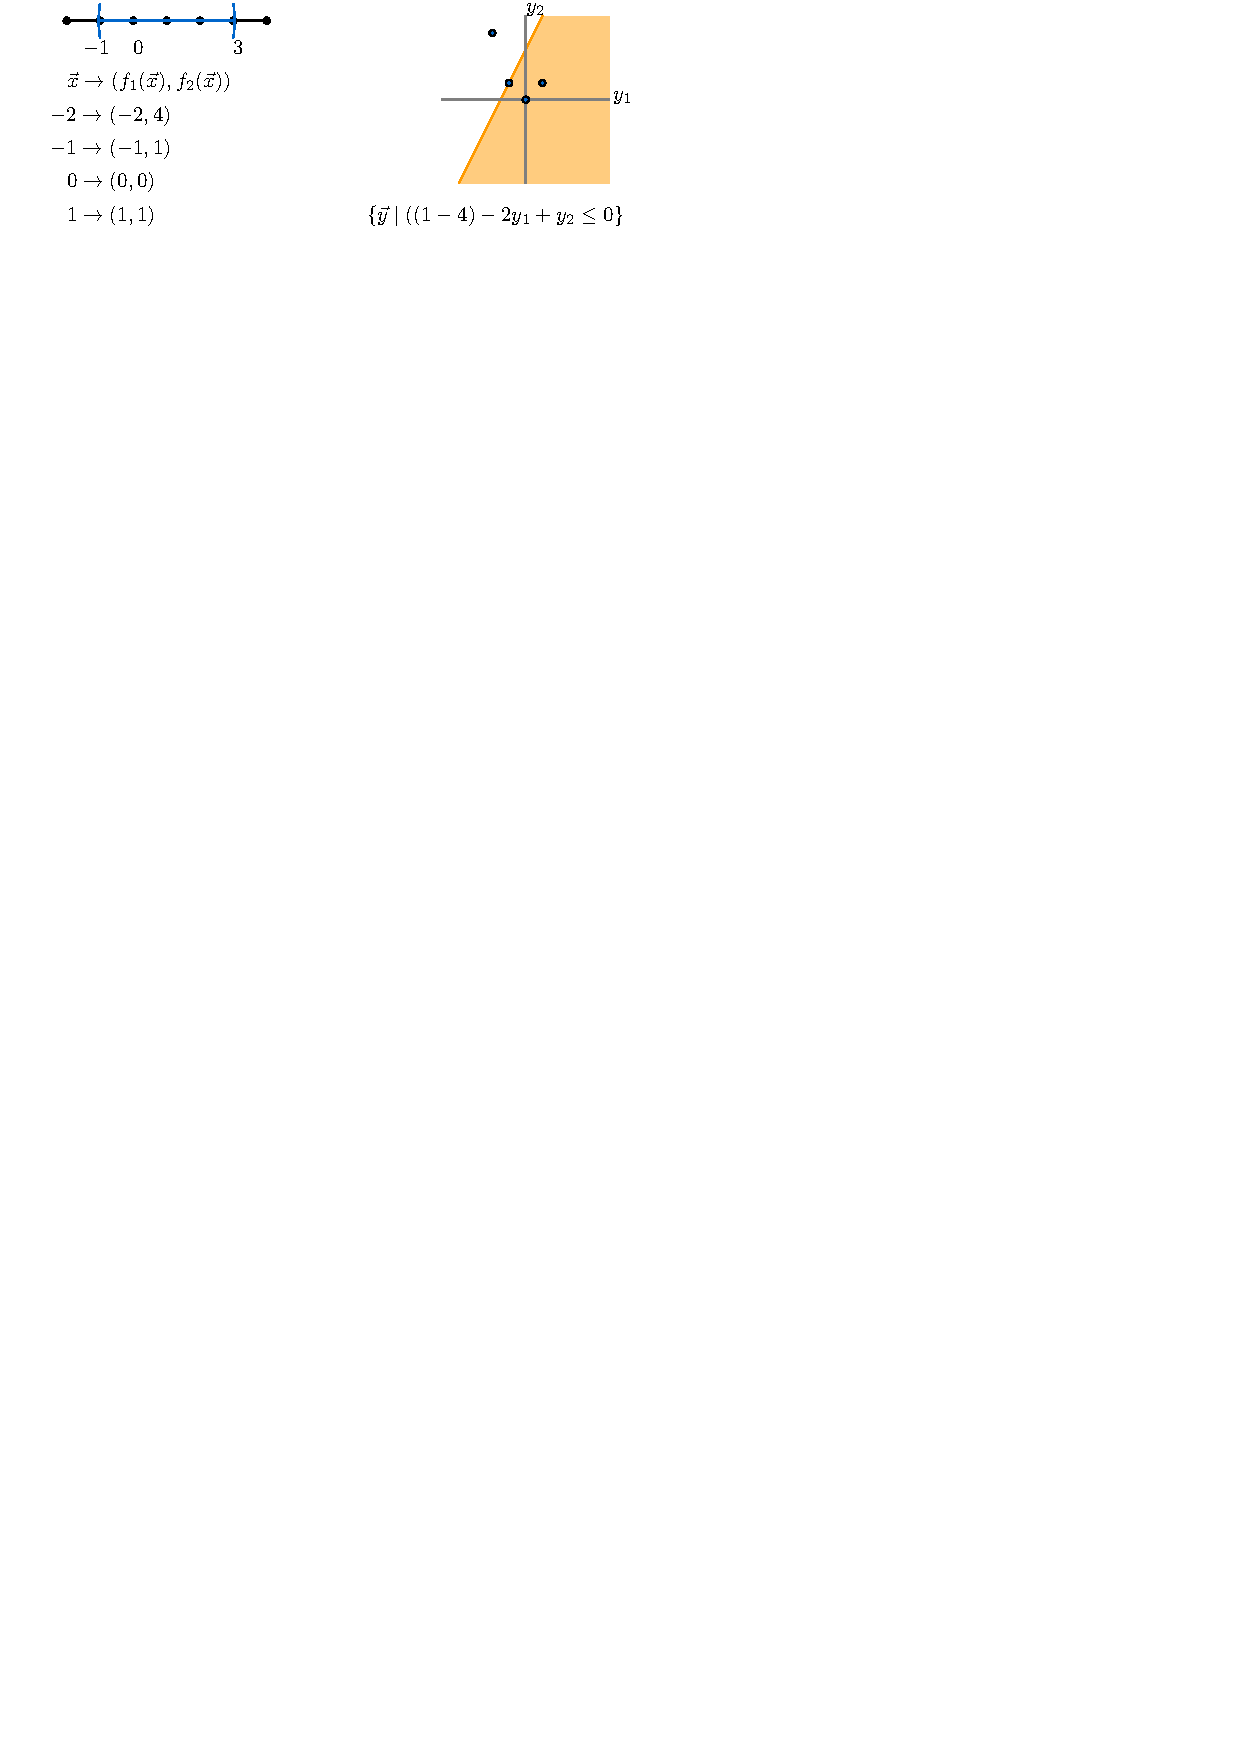
\includegraphics{../algebraic}
    \caption{algebra}
    \label{fig:algebraic}
\end{figure}


\begin{proof}[Proof of Lemma~\ref{lemma:uncertain_intersection}]
This proof is illustrated by Figure~\ref{fig:pointline}.
For each edge $e \in U$ with corresponding reflex vertex $v$, we know that the line $qv$ intersects the line $\ell_e$ supporting $e$ on the domain of $e$ (this property is guaranteed by the construction of Aronov \etal). Per construction, we know that the point $q$, lies below the line $\rho$, and the second level of our data structure guarantees that the intersection point between $qv$ and $\rho$ lies on the trajectory of $r$. It follows that $q$ can see $r$ if and only if, the intersection point $(x,y)$ between $qv$ and $\ell_e$ lies above $\rho$. Given $\rho, q, v$ and $\ell_e$, we can algebraically compute this intersection point $(x,y)$. We then substitute the equation for $(x, y)$ into the equation for $\rho$ and the point $(x,y)$ lies above this line if and only if the result is greater than $0$:

\[
vq := \left\{x,y \mid 0 =  \frac{x_4 - a_4}{x_3 - a_3} x - \frac{x_4 - a_4}{x_3 - a_3}x_3 + x_4  \right\}
\]

The lines $vq$ and $\ell_e$ intersect at the point where their $y$-coordinate is equal so it follows that: 


\begin{align*}
    x_1 x - x_2 =  \frac{x_4 - a_4}{x_3 - a_3} x - \frac{x_4 - a_4}{x_3 - a_3}x_3 + x_4 \\
    (x_3 - a_3)(x_1 x - x_2) = (x_4 - a_4) x - (x_4 - a_4)x_3 + (x_3 - a_3) x_4 \\
    (x_3 - a_3)x_1 x - (x_4 - a_4) x = x_2 (x_3 - a_3) - (x_4 - a_4)x_3 + (x_3 - a_3) x_4 
\end{align*}

\begin{figure}[h]
    \centering
    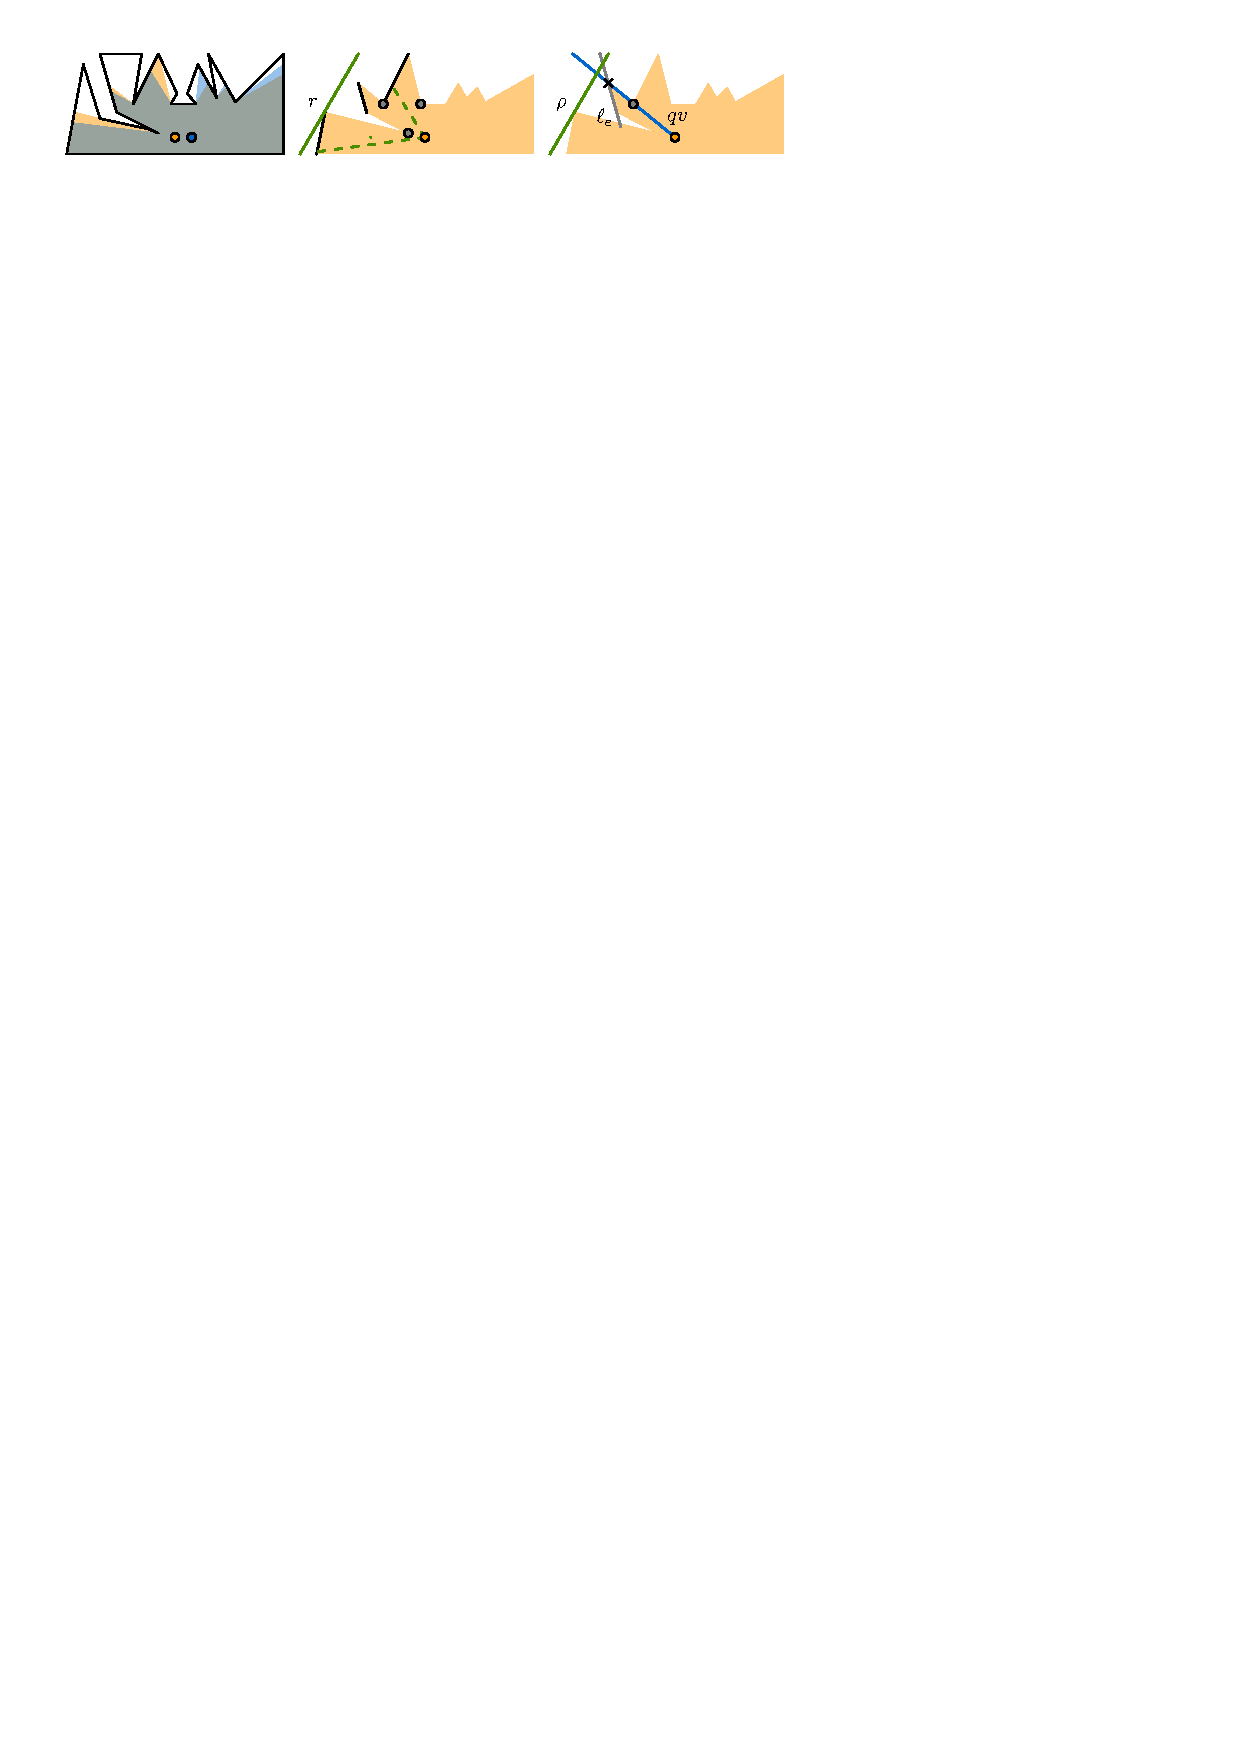
\includegraphics[]{../pointline}
    \caption{ (left) Two points in orange and blue, which have the same implicit visibility polygon, however there could be several placement of $r$ such that $r$ only intersects one of the two explicit visibility polygons. (middle) Entity $r$ in green, $q$ in orange and the chain of uncertain edges. (right) An illustration of the geometric argument. We compute the intersection between $\ell_e$ and $qv$ and check if that point lies below or above $\rho$.}
    \label{fig:pointline}
\end{figure}


From this equation we can extract the coordinates of the intersection point $(x,y)$ between $vq$ and $\ell_e$:

\begin{align*}
    x = \frac{x_2 (x_3 - a_3) - (x_4 - a_4)x_3 + (x_3 - a_3) x_4}{ (x_3 - a_3)x_1 - (x_4 - a_4)} \\
    y = x_1 \frac{x_2 (x_3 - a_3) - (x_4 - a_4)x_3 + (x_3 - a_3) x_4}{ (x_3 - a_3)x_1 - (x_4 - a_4)} - x_2
\end{align*}

Lastly we substitute the algebraic expression for $(x,y)$ into the formula for $\rho$ and we rewrite this expression to fit the predicate form by Agarwal \etal \cite{agarwal2013range}:

\begin{align*}
    0 \ge a_1 (x_2 (x_3 - a_3) - (x_4 - a_4)x_3 + (x_3 - a_3) x_4) - \\
    x_2 - x_1 (x_2 (x_3 - a_3) - (x_4 - a_4)x_3 + (x_3 - a_3) x_4) + x_2 \\
    0 \ge [-a_1 a_3] (x_2) + [a_3]( x_1 x_2) + [a_1] (x_2 x_3) + [a_1a_4] (x_3) + \\
    [- a_4] (x_1 x_3) + [- a_1 a_3]( x_4) + [a_3] (x_1 x_4) + [-1](x_1 x_2 x_3)
\end{align*}

Thus we found a predicate $F(\vec{x}, \vec{a})$ with:

\begin{align*}
    (f_1, f_2, f_3, f_4, f_5, f_6, f_6, f_8) = (x_2, x_1x_2, x_2x_3, x_3, x_1x_3, x_4, x_1x_4, x_1x_2x_3) \\
    (g_0, g_1, g_2, g_3, g_4, g_5,g_6, g_7,g_8) = (0, -a_1a_3, a_3, a_1, a_1a_4, -a_4, -a_1a_3, a_3, -1)
\end{align*}

It follows that we can map every uncertain edge plus its reflex vertex to a point in $\mathbb{R}^8$ using the $f$-maps provided by the predicate. Any query consisting of the line $\rho$ and the point $q$ gets mapped to a halfspace in $\mathbb{R}^8$. The line $\rho$ (and with it, the trajectory of $r$) intersects an edge in $U$ if and only if its representative point lies in this halfspace. 
\end{proof}



\begin{proof}[Proof of Lemma~\ref{lemma:hyperbola}]
Recall that we required that entity $q$ walks from $(a_1, a_2)$ to $(a_1 + a_3, a_2 + a_4)$ and that entity $r$ walks from $(a_5, a_6)$ to $(a_5 + a_7, a_6 + a_8)$. We can parametrize the position of entity $q$ and $r$ on the time $t$ as follows:

\begin{equation}
    \label{eq:line}
     q(t) = \left( \begin{array}{c}
         x_{q(t)}  \\
         y_{q(t)} 
    \end{array}  \right) = 
    \left( \begin{array}{c}
         a_1 + a_3 t \\
         a_2 + a_4 t
    \end{array}  \right)  \quad
      r(t) = \left( \begin{array}{c}
         x_{r(t)}  \\
         y_{r(t)} 
    \end{array}  \right) = 
    \left( \begin{array}{c}
         a_5 + a_7 t \\
         a_6 + a_8 t
    \end{array}  \right) 
\end{equation}


At all times, the line $\gamma(t)$ represents the line through $q(t)$ and $r(t)$. We say that at all times, $\gamma(t)$ has slope and offset $(\alpha(t), \beta(t))$. The parametrisation of $\gamma(t)$ then becomes:

\begin{equation}
\label{eq:curve}
   \gamma(t) = \left( \begin{array}{c}
         \alpha(t)  \\
         \beta(t) 
    \end{array}  \right) = 
    \left( \begin{array}{c}
         \frac{y_{r(t)} - y_{q(t)}}{x_{r(t)} - x_{q(t)}}  \\
         \alpha(t)\cdot x_{q(t)} - y_{q(t)}
    \end{array}  \right) =
    \left( \begin{array}{c}
         \frac{ a_6 - a_2 + (a_8 - a_4) t}
      { a_5 - a_1  + (a_7 - a_3) t }  \\
         \alpha(t) (a_1 - a_3 t) - a_2 - a_4 t 
    \end{array}  \right)
  \end{equation}
  
  If the time $t$ lies between $0$ and $1$, this parametric equation traces our hyperbolic segment. If we take $t$ over all of $\mathbb{R}$, the parametric equation traces a full hyperbola. For reasons that will become apparent later, we opt to rewrite the hyperbolic curve to a canonical form that drops the dependence on $t$. First we take the formula for the $\beta$-coordinate and isolate $t$:
  
  \[
     t = \frac{\alpha(t) a_1 - a_2  - \beta(t)}{\alpha(t) a_3 + a_4}
  \]
We then take the formula for the $\alpha$-coordinate and remove the fraction by multiplying both sides with $ ((a_5 - a_1)  + (a_7 - a_3) t)$:

\[ 
\alpha(t)(a_5 - a_1)  + \alpha(t)(a_7 - a_3) t = (a_6 - a_2) + (a_8 - a_4) t
\]

We substitute the value for $t$ into this equation, and remove the fraction by multiplying both sides with $(\alpha(t) a_3 + a_4)$:

\begin{align*}
\alpha(t)(\alpha(t) a_3 + a_4)(a_5 - a_1)  + \alpha(t)(a_7 - a_3) (\alpha(t) a_1 - a_2  - \beta(t)) = \\
(a_6 - a_2)(\alpha(t) a_3 + a_4) + (a_8 - a_4) (\alpha(t) a_1 - a_2  - \beta(t)) \Rightarrow \\
\alpha(t)^2a_3(a_5 - a_1) + \alpha(t)a_4(a_5 - a_1)  + \alpha(t)^2a_1(a_7 - a_3)
- \alpha(t)a_2(a_7 - a_3)  - \alpha(t)\beta(t)(a_7 - a_3) = \\
\alpha(t) a_3(a_6 - a_2) + a_4(a_6 - a_2) + \alpha(t)a_1(a_8 - a_4) - a_2 (a_8 - a_4) - \beta(t)(a_8 - a_4) 
\end{align*}

Lastly, we take all variables to one side and we group on terms based on $\alpha$ and $\beta$ and we remove redundancies

\begin{align}
\label{eq:hyperbola}
    0= [\alpha(t)^2](a_5 a_3 -2 a_1 a_3 + a_1 a_7)+ \\
    [\alpha(t)](a_4 a_5 - a_3 a_6 + a_2 (2 a_3 - a_7) - a_1 a_8) + \\
    [\alpha(t)\beta(t)](-(a_7 - a_3)) + [\beta(t)](-(a_8 - a_4)) + [1](a_4(a_6 - a_2)- a_2 (a_8 - a_4))
\end{align}
\end{proof}


\end{document}